% This file is part of the causal-kepler project
% Copyright 2013, 2014 the authors.

% # to-do
% - write causal description

\documentclass[12pt, preprint]{aastex}

\usepackage{graphicx}
\usepackage{subfigure}
\usepackage[normalem]{ulem}
%\usepackage{caption} 
%\usepackage{subcaption} 
\usepackage{epstopdf}
\usepackage{color}
\usepackage{hyperref}
\usepackage{url}

\usepackage{natbib}

%\graphicspath{{figures/png/}}

\newcommand{\notenglish}[1]{\textit{#1}}
\newcommand{\sic}{\notenglish{sic}}
\newcommand{\project}[1]{\textsl{#1}}
\newcommand{\Kepler}{\project{Kepler}}
\newcommand{\name}{CPM}
\newcommand{\set}[1]{\mathcal{#1}}
\newcommand{\given}{\,|\,}
\newcommand{\todo}[1]{\textbf{#1}}
\newcommand{\revise}[1]{\textcolor{green}{#1}}
\newcommand{\remove}[1]{\sout{#1}}

\newcommand{\Bernhard}[1]{$\bullet$\footnote{{\bf Bernhard:} #1}}
\newcommand{\Dun}[1]{$\bullet$\footnote{{\bf Dun:} #1}}

\bibliographystyle{apj}
\definecolor{linkcolor}{rgb}{0,0,0.5}
\hypersetup{colorlinks=true,linkcolor=linkcolor,citecolor=linkcolor,
            filecolor=linkcolor,urlcolor=linkcolor}

\begin{document}

\title{ \remove{Calibrating the pixel-level Kepler imaging data with a causal data-driven model\\}
  \revise{
  A Causal, Data-Driven Approach to Modeling the Kepler Image Data
 \\ }
}
\author{%
  Dun~Wang\altaffilmark{\ref{CCPP}},
  David~W.~Hogg\altaffilmark{\ref{CCPP},\ref{CDS},\ref{MPIA},\ref{email}},
  Daniel~Foreman-Mackey\altaffilmark{\ref{UW},\ref{SF}},
  Bernhard~Sch\"olkopf\altaffilmark{\ref{MPIIS}}
  }
\newcounter{address}
\setcounter{address}{1}
\altaffiltext{\theaddress}{\stepcounter{address}\label{CCPP}%
  Center for Cosmology and Particle Physics, Department of Physics, New York University}
\altaffiltext{\theaddress}{\stepcounter{address}\label{CDS}%
  Center for Data Science, New York University}
\altaffiltext{\theaddress}{\stepcounter{address}\label{MPIA}%
  Max-Planck-Institut f\"ur Astronomie, Heidelberg, Germany}
\altaffiltext{\theaddress}{\stepcounter{address}\label{email}%
  To whom correspondence should be addressed; \texttt{<david.hogg@nyu.edu>}.}
\altaffiltext{\theaddress}{\stepcounter{address}\label{MPIIS}%
  Max-Planck-Institut f\"ur Intelligente Systeme, T\"ubingen}
\altaffiltext{\theaddress}{\stepcounter{address}\label{UW}%
 Astronomy Department, University of Washington, Seattle, WA 98195}
\altaffiltext{\theaddress}{\stepcounter{address}\label{SF}%
Sagan Fellow}


\begin{abstract}
Astronomical observations are affected by several kinds of noise, each with its own causal source; 
there is photon noise, stochastic source variability, and residuals coming from imperfect calibration of the detector or telescope. 
The precision of NASA \Kepler\ photometry for exoplanet science---% no spaces around ---
the most precise photometric measurements of stars ever made---%
appears to be limited by unknown or untracked variations in spacecraft pointing and temperature, 
and unmodeled stellar variability. Here we present the Causal Pixel Model (\name) for \Kepler\ data, 
a data-driven model intended to capture variability but preserve transit signals. 
The \name\ works at the pixel level so that
it can capture very fine-grained information about the variation of the spacecraft.
\remove{The \name\ predicts each target pixel value from a large number of pixels of other stars sharing the instrument variabilities 
while not containing any information on possible transits in the target star.} \revise{The CPM models the systematic effects in the time series of a pixel using the pixels
around many other stars and the assumption that any shared signal in
these causally disconnected light curves is caused by instrumental
effects.} In addition, we use the target star's future and past (auto-regression). 
By appropriately separating, for each data point, the data into training and test sets, 
  we ensure that information about any transit will be perfectly isolated from the model. 
The method has four \remove{hyper-parameters (the number of predictor stars, the auto-regressive window size, 
and two L2-regularization amplitudes for model components),}
\revise{tuning parameters---the number of predictor stars, the auto-regressive window size, 
and two L2-regularization amplitudes for model components,}
 which we set by cross-validation. 
We determine a generic set of \remove{hyper-parameters}\revise{tuning parameters} that works well for most of the stars and apply the method to a corresponding set of target stars.
\remove{We find that we can consistently outperform (for the purposes of exoplanet detection) 
  the \Kepler\ Pre-search Data Conditioning (PDC) method for exoplanet discovery.} 
\revise{We find that \name\ can consistently produce relatively low-noise (CDPP) light-curves. In this paper, we demonstrate that pixel-level de-trending is possible while retaining transit signals (with a train-and-test framework) and we think that methods like \name\ is generally applicable and might be useful for  K2, TESS, etc, where the data aren't these clean postage stamps like \Kepler.}


\end{abstract}

\section{Introduction}

The photometric measurements of stars made by the \Kepler\ \remove{satellite}\revise{space craft} are precise enough
  to permit discovery of exoplanet transits with depths smaller than $10^{-4}$.
This precision results from great spacecraft stability,
  supplemented by various methods for removing small residual spacecraft-induced and stellar-variability trends in the brightnesses,
  either filtering the data (with things like median filters)
  or fitting the data with flexible models (like polynomials or splines or Gaussian Processes; 
  \cite{gaussian}).
When employed in the service of exoplanet search and characterization,
  these methods are usually agnostic about whether photometric variations originate in the spacecraft or in the star itself;
  that is, they obliterate intrinsic stellar variability along with spacecraft issues.

In general, there are many reasons for apparent photometric variability in a \Kepler\ source.
There is intrinsic stellar variability,
  which is of interest to some and a nuisance to others.
There is also variability of overlapping fainter stars;
  that is, confusion noise combined with variability of the confusing sources.
There are small changes in spacecraft pointing,
  which leads to slightly different illumination of the focal-plane pixels,
  and thus different sensitivity to variations in the device.
There are also \emph{intra-pixel} sensitivity variations that can contribute, which was first measured by \revise{\cite{subpixel}}.
There are small changes in spacecraft temperature,
  which lead to point-spread function (PSF) and differential \remove{(across the focal plane)} pointing changes.
These also lead to changes in pixel and intra-pixel illumination.
Stellar proper motion, geometric parallaxes, and differential stellar aberration as the spacecraft orbits all do more of the same.
There is electronic cross-talk between detectors and charge-transfer inefficiency;
  these can effectively transfer variability from one source to another.
There are additional electronics effects like ``rolling bands'' that put additional features into light-curves \revise{\citep{handbook}}.
There are also \remove{probably} changes to the detector sensitivity with temperature and time,
  possibly illimunation-history effects,
  and possibly sources of variability not yet considered.
The remarkable thing about \Kepler\ is that it is trying to measure stars at a level of precision
  much higher than ever previously attempted;
  new effects really \emph{must} appear at some point.
In \figurename~\ref{ccd}, we show the pixel-level variability in the \Kepler\ data
  near one bright star that shows minimal intrinsic variability;
  this figure highlights the spacecraft-induced effects.

\remove{We propose and advise dealing with}\revise{We propose to deal with} these variations in \Kepler\ light-curves by \emph{modeling} them.
In this context, a model is \remove{(at least)} a parameterized function that can predict data, given parameter settings,
  and an objective function that can be used to set or sample those parameters.
In some cases, the objective function can be given a probabilistic justification or interpretation, e.g., if it is constructed using a likelihood and a prior pdf.
The model can be a physical model (of the spacecraft PSF, pointing, temperature, and so on)
  or it can be a flexible, effective model that has no direct interpretation in terms of physical spacecraft parameters.
If done well, we would expect a physical model to do a better job,
  because it embodies more prior information,
  but it requires research and intuition about dominant effects. 
If this research and intuition is wrong or incomplete, a physical model may actually perform worse.
The model we propose here is in the non-physical, effective category.
The \Kepler\ community is familiar with these kinds of models;
  to our knowledge, \emph{all} successful light-curve ``de-trending'' methods
  are flexible, effective models.

One such method---one that is designed to describe or model spacecraft-induced problems
  but \emph{not} interfere with measurements of stellar variability---%
  is the \Kepler\ Presearch \remove{(\sic)} Data Conditioning (PDC, \cite{pdc1}).
The PDC builds on the idea that systematic errors have a temporal structure that can be extracted from ancillary quantities. 
%This seems the original paper on PDC:
%[PDC1] https://kepler.nasa.gov/science/ForScientists/papersAndDocumentation/SOCpapers/7740-67-pdc-jtwicken-copyright.pdf
%
%This describes the later version of PDC:
%[PDC2] http://arxiv.org/pdf/1203.1382v1.pdf
%[PDC3] http://arxiv.org/pdf/1203.1383v1.pdf

In the first PDC \citep{pdc1}, 
  removal of systematic errors was performed based on correlations with a set of ancillary engineering data. 
These data include the temperatures at the local detector electronics below the CCD array, 
  and polynomials describing the centroid motion of the targets from PA\revise{(Photometric Analysis)}.

In \cite{pdc2,pdc3}\remove{, filtered light-curves of other stars are used instead. 
The light-curve of a target star is projected on the leading eight principal components of these light-curves. 
This projection is then removed from the star's light-curve. 
The principal components are computed from a set of relatively quiet stars close in position and magnitude. 
This was done since it was observed that otherwise, too much of the stellar variability was being removed.}

\revise{In the most recent version of PDC (PDC-MAP, \cite{pdc2,pdc3}), filtered light-curves of other stars are used
instead. Using a set of relatively quiet stars on each detector, the
top 8 principle components are computed for every quarter of Kepler
data. The maximum a posteriori linear combination of these basis light
curves---computed using an empirical prior on the trend
magnitudes---are used to model and remove the systematics in all the
Kepler light curves. The choice to use such a small number of
components and to apply priors was made in order to reduce
over-fitting and retain physical signals after systematics removal.}

\remove{From the point of view of the present paper, 
one can only guarantee that {\em no} stellar variability is removed if the stars do not depend on time at all.
If both the target star signal as well as some of the other stars do depend on time, 
  then time acts as a confounder influencing both, and thus the true signals are not statistically independent, 
  and thus the target signal may be compromised. 
We suspect that this effect is limited in} \cite{pdc2,pdc3}, 
  \remove{since only eight principal components are used, which limits the capacity of the model.}

PDC \remove{``de-trends''}\revise{"co-trends" or calibrates} the \Kepler\ light-curves by removing those parts that are explained by the basis light-curves
  generated from a principal components analysis (PCA) of filtered light-curves.
That is, it exploits statistical dependences between different time series, regularizing the fit (and avoiding over-fitting) 
  by filtering and restricting the dimensionality (through PCA).

The method proposed here, \name, shares the motivation of PDC.
The main differences are that
\begin{enumerate}
\item
\name\ works in the pixel domain, not the light-curve domain, so it has access to more fine-grained information
\item
\name\ has far more freedom (far more parameters) than the PDC
  but it strictly avoids over-fitting the light-curves on exoplanet-transit time-scales
  through strong regularization and a train-and-test framework. 
  \revise{PDC mitigates overfitting by
reducing the freedom of the model and applying empirical priors to the
fit coefficients.}
\item 
\name\ directly optimizes for prediction accuracy, while PDC uses PCA projections.
\item
\remove{the purpose of \name\ is to search for exoplanets, so in \name, intrinsic stellar
  variability is also removed as well as the systematics.}
  \revise{The current version of \name\ is
tuned to remove systematics while minimizing the impact on exoplanet
transit signals. It makes no attempt to retain lower frequency signals
that can be produced by other astrophysical signals.}
\item 
\name\ uses as inputs only instantaneous values of other stars, plus near future and past of the star itself in an autoregressive fashion, while PDC works with time series (light-curves) of the other stars.
\end{enumerate}

The two methods (\name\ and PDC) are similar however,
  in that they both make the \remove{(implicit or explicit)} assumption that whatever spacecraft effects are imprinting variability on a stellar light-curve
  must also be imprinting similar or related variability on other light-curves.
\remove{In their current versions, they also assume that the relationships can be captured with linear models (although we have also used nonlinear predictions methods for \name, which would be harder to do in PDC).}
By going to the pixel level (unlike the PDC, which works at the photometry level),
  \name\ makes it easier for the model to capture variability
  that is coming through variations in the centroids and point-spread function
  from spacecraft pointing, roll, and temperature.

Before we start, a few reminders about the \Kepler\ data are in order:
The \remove{satellite}\revise{space craft} \remove{always observes}\revise{observed} precisely the same field, at fixed pointing (as closely as possible).
\revise{About 6\% of the 96,465,600 pixels}\remove{Only a few percent of the 80 million pixels} in the focal plane are telemetered down
  to Earth from each 30-min exposure;
  the telemetered pixels are associated with \Kepler\ target stars chosen for study by the \Kepler\ Team \revise{(along with a non-trivial set collateral pixels used for calibration)}.
The \remove{satellite}\revise{space craft} is rolled by 90~deg every \remove{90-ish}\revise{93} days (to satisfy Solar-Angle constraints).
The focal plane contains many CCDs;
  this plus the 90-deg rotations means that each star is at a particular location
  on a particular CCD for \remove{90-ish-day}\revise{quarter} contiguous periods of time.
The PSF varies strongly across the field and is badly sampled.
The stars span a huge range in brightness;
  some of \Kepler's most important targets even saturate the device and bleed charge.
The stellar photometry returned by the \Kepler\ SAP and PDC pipelines is based on
  straight, \emph{unweighted} sums of pixels in small patches centered on the stellar centroid.
We will return to this latter point at the end;
  this kind of photometry cannot be optimal;
  it must be possible to do a better job with the photometric measurements.
That's beyond the scope of this project but a place for a valuable intervention on the \Kepler\ data.

\remove{The scope of this project is an intervention---\name---that makes the \Kepler\ transit photometry more precise.}

We describe the method and deliver all the relevant code in a public, open-source repository.
We also provide an interface to the \Kepler\ data that \remove{delivers improved ``\name\ photometry''}\revise{can be used
to produce ''\name\ photometry''}
  for every \Kepler\ target.

\section{Causal data-driven model}

The first general idea about data-driven modelling of the kind used here
  is that each data point or data source is going to be 
  \emph{predicted} with or using a parameterized mathematical function of \emph{other data}.
That is, given a choice of some \emph{target} \Kepler\ data,
  we are going to find parameters of a function that takes as input some of the other \Kepler\ data,
  and provides as output predictions of the target data.
The simplest models are \emph{linear models},
  in which predictions for the target data are built from linear combinations of the other data,
  and in which the objective functions are quadratic in the prediction residual.
Examples of quadratic objective functions include Gaussian likelihoods, mean-squared-error, and chi-square statistics.
These models are simple,
  not just because they are easy to express and compute,
  but because optimization is convex:
There is only one optimum for the objective function.

The point of these models is to be \emph{flexible},
  so the usual approach is to make the input data set very large,
  and the number of parameters large,
  often as large as---or larger than---the target data available.
Such fits require \emph{regularization} to break degeneracies
  and control ill-constrained parameters.
These regularizations do for optimizations what priors do for posterior probability inferences;
  they express the desired behavior of the fit in the absence of data
  or along directions in parameter space in which the data are not constraining.
General regularizations or priors will break the convexity of linear model fitting;
  if convexity is to be maintained, these regularizations also have to be quadratic,
  or else one of a class of other known forms (one of which is L1-regularization).
Given these considerations, it makes sense to try to build our pixel-level model
  using a linear model with a quadratic objective function and a quadratic regularization;
  this is what \name\ will be.

The second general idea about data-driven modelling is the investigator's beliefs about the causal processes that generate the data are crucial in restricting the kinds of data that can be used as input to the model.
That is, different assumptions about the physical properties of the data and the data-taking system lead to different structures for the data-driven model.
In the case of \Kepler\ data, 
  if we examine two arbitrary stars far away from each other 
  on the same CCD as in Fig~\ref{ccd} (every grid in the plot is a pixel light-curve time series), 
  we can obviously see that the two stars that are hundreds pixel away from each other do have similar trends. 
  If we believe that different stars in the \Kepler\ field vary independently 
  (that is, are not physically synchronized in any way) because of the distance between them, 
  then the only reason that one star might show variability that is strongly \emph{predictive} (useful for prediction) of another star's variability
  is that both stars are being observed by the same device or spacecraft.
That is, one star's pixels can be used to predict another star's pixels inasmuch as spacecraft issues imprint on both stars in related ways;
  they share a common cause---the systematics.  
For another example, if we think the spacecraft is being affected by
  processes that take place over time-scales longer than a single read-out
  (for example, thermal processes),
  then it would be sensible to model the data at time $t$ using not just simultaneous data, but also data from a range of times around $t$.
For another example, if an investigator doesn't care about preserving stellar variability,
  and just wants to detect exoplanet transits (say),
  pixels from the target star can be used to predict pixels from the target star,
  provided they are at large-enough time lags that they don't contain information about
  the signals of interest (i.e., the transits).
That is, if the model is designed to fit not just spacecraft variability
  but also intrinsic stellar variability,
  the predictive model will be permitted to use as input pixels that \emph{do} overlap the target star.
In what follows, we are going to use input data both from pixels of other stars and the target star pixels' past and future.
These models ought to remove both spacecraft variability and intrinsic stellar variability, which is \remove{optimal}\revise{optimized} for exoplanet transit searching.

\begin{figure}[p]
\begin{center}
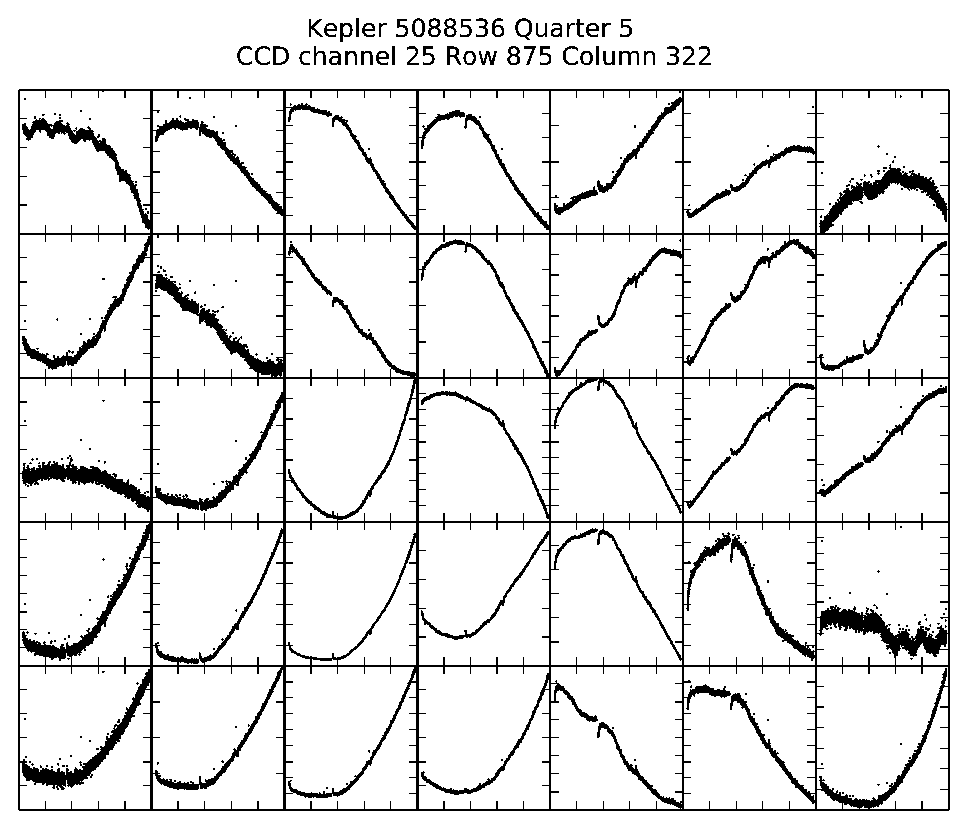
\includegraphics[width=0.4\textwidth]{f1a}
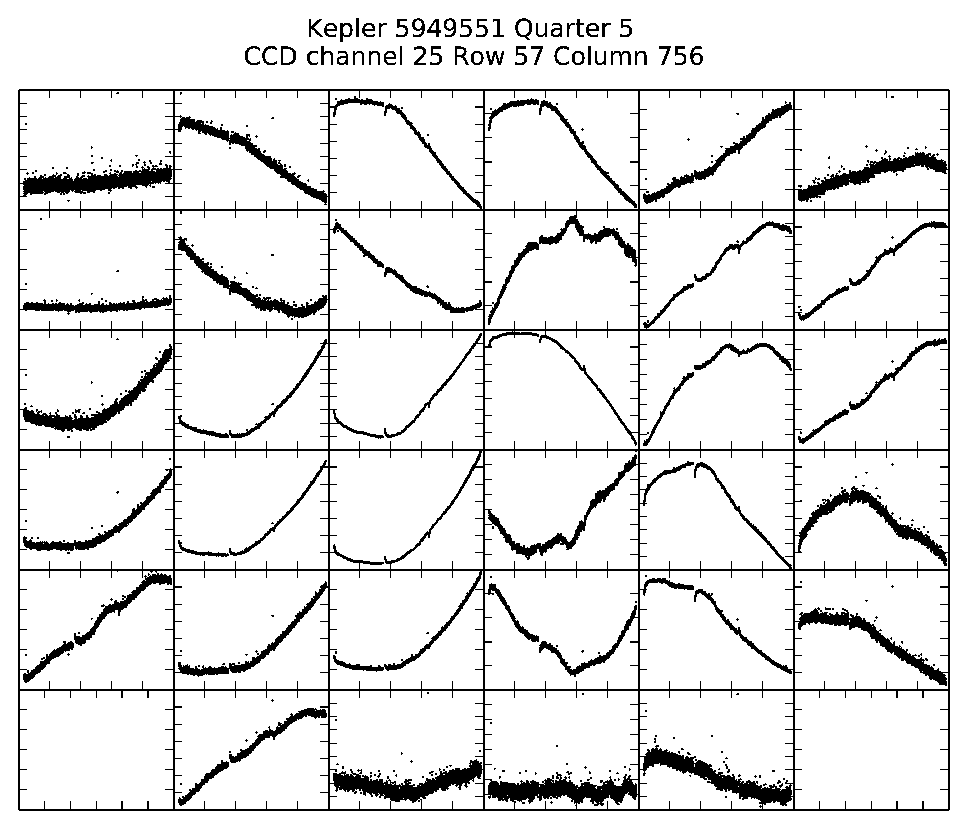
\includegraphics[width=0.4\textwidth]{f1b}
\end{center}
\caption{
  \label{ccd} 
  Stars on the same CCD share systematic errors. 
  The two panels show pixel fluxes (brightnesses) for two stars in quarter 5. \emph{Left:} KIC 5088536, \emph{Right:} KIC 5949551; 
  here, KIC stands for Kepler Input Catalog. Both stars lie on the same CCD, 
  but far enough apart such that there is no stray light from one affecting the other. 
  Each panel shows the pixels contributing to the respective star.
  Note that there exist similar trends in these two stars, caused by systematic errors. 
%The idea of our approach is to predict each pixel from a set of pixels from other stars in order to remove those systematics.
}
\end{figure}

The third general idea is that we need to control for over-fitting.
That is, once you have a flexible-enough model you can in principle fit \emph{anything},
  whether it was caused by the spacecraft, intrinsic stellar variability, or a transiting exoplanet.
How do you prevent a very flexible model from taking small noise-induced fluctuations in all the input data
  and carefully combining them linearly into detailed models for every nook and cranny in the target data?
In most projects in astrophysics, over-fitting is controlled for by limiting model freedom.
The model is restricted in the number of parameters
  (as in ``you can't have more parameters than data points'')
  or by limiting the dimensionality
  (as in principal components analysis)
  or by applying strong priors
  (as with smoothness priors or regularization, 
  that effectively reduce freedom without explicitly reducing the number of parameters).
In each case, the restriction on model freedom is controlled by some \emph{\remove{hyper-parameter}\revise{tuning parameters}}
  (such as the number of inputs, or number of principal components, or the strength of the smoothness prior).
The \remove{hyper-parameters}\revise{tuning parameters} can be set or tested with tools like cross-validation,
  the fully marginalized likelihood (Bayes factor or evidence),
  chi-squared statistical criteria,
  or intuition or heuristics.
Here we take a different and more general approach, which is to use a train-and-test framework.

In this framework, the data used to \emph{train} the model%
  ---meaning set the values of the parameters of the model---%
  are disjoint from the \emph{test} data
  ---meaning the data that are being predicted (the target data).
Because we are concerned with detecting exoplanet transits,
  which take few hours,
  we adopt an extreme version of the train-and-test framework,
  in which the training data are always separated from the test data by couple of hours.
That is, when we are using the model to predict a particular pixel in the target data taken at time $t$,
  we use parameters obtained by an optimization that makes use of only data
  that comes either at times prior to $t-\Delta t$ or after $t+\Delta t$,
  where $\Delta t$ is a tunable parameter but which we will set to $9$~h.
This ensures that no information about any exoplanet transit itself
  can be entering into the prediction of the pixels contributing to the stellar photometry.
In general, if there is a scientific goal of preserving intrinsic stellar variability,
  or transit signals,
  on time-scales of $\tau$,
  the parameter optimization ought to be based on training data taken with a time-exclusion zone of half-width $\Delta t > \tau$.

In addition, 
  each training data set within which we set the parameters (by optimization) has a finite total time extent $t_{\max}\approx 30$\,d.
The train-and-test framework, which includes data out to time $t_{\max}$ but excludes data within $\Delta t$ of the test data,
  effectively assumes that the signals worth preserving have time-scales less than $\Delta t$ 
  but don't recur on time-scales shorter than $t_{\max}$.
Those assumptions are good for our purposes but not necessarily ideal for all users:
Short-period exoplanets and certain kinds of stellar variability
  could be wiped out by a model with these settings of the training-data regime.

The fourth general idea involved in this kind of data-driven modelling is that the models often aren't \emph{interpretable}, 
  or at least are hard to interpret.
This means, in particular, that although the model might do a good job of \emph{predicting} the target pixels,
  using a linear (or more complex) combination of the input pixel data,
  it won't deliver anything that can be unambiguously interpreted as the \emph{flux} of the star in question,
  or any other signal we care about.
The data-driven model \emph{effectively} describes the pointing, point-spread function, and flat-field
  of the telescope and camera,
  plus the variability of every star and every exoplanet transit,
  but it does so without ever \emph{explicitly} creating any of those objects.
We have to make some kind of heuristic or interpretive move to extract from the data-driven model the quanitites of interest.

Finally, the fifth general idea is that there is no objective \emph{ground truth} against which we can tell
  that any particular data-driven model is better or worse than any other.
This problem is a problem for \name, and for the \Kepler\ PDC, and any other data-driven calibration models.
One might think that the ``best'' model is the one that predicts data with lowest variance;
  this would be true if all models adhered to the same train-and-test framework, which they don't.
Besides, a model that can predict not just the spacecraft-induced variability,
  but also variability caused by exoplanet transits of interest,
  will effectively over-fit and distort the most important information in the light-curves.
That is, what is considered best for modelling the data depends on the objectives of the user.
For us, who are interested (in the long term) in finding and characterizing Earth analogs,
  the ``best'' data-driven model is the one that produces the most success in finding and characterizing Earth analogs!
What we will show in what follows is that the \name\ photometry does not distort
  artificial exoplanet transit signals injected into real \Kepler\ pixel-level data
  and promising properties of the \name\ outputs \revise{on real Kepler light-curves}.
In the end, the value of the \name\ will be demonstrated by the scientific projects it enables.

We also want to emphasis that all the calibration in this paper for \Kepler is 
  based on the assumption that the device is \remove{'self-calibratable'}\revise{can be self-calibrated}, 
  which means all the information we need to calibrate the device are contained in the device itself 
  (either in science data or engineering data) and no external information, 
  for example, measurements from other device, are needed.
  And a description of the method in the machine learning context can be found in \cite{icml2015}

\section{\name\ specification and \revise{tuning parameters}}
\subsection{\name\ model}
Each individual \Kepler\ target star is, for each quarter (each \remove{90-ish-day})
  on a particular CCD on the \Kepler\ focal plane.
Associated with each target star is some set of pixels,
  located in a small contiguous patch \remove{more-or-less} centered on the target star,
  and telemetered down once for every 30-min exposure.
Here we are ignoring all short-cadence data that is taken in a different mode with shorter exposures.
That is, each telemetered pixel in each CCD is associated with a particular \Kepler\ target star.

Let's consider a particular pixel $m$ in the focal plane in one particular month
  (here we always use data per month rather than quarter,  since there are discontinuities between every \remove{30-ish-day period}\revise{month}).
In that month, the spacecraft delivers $N\sim 1300$ measurements $I_{m,n}$
  of the intensity falling in pixel $m$ at the $N$ times $t_n$ at which exposures were taken during the month.
(For intensity measurements $I_{m,n}$ here we are using pixels from \revise{the FLUX column of Target Pixel File, which is flux of each pixel after processed by the pipeline module CAL, the removal of the interpolated background, and the removal of cosmic rays} on MAST
  \footnote{\url{http://archive.stsci.edu/kepler/}}, for details of the TPF, 
  see the \project{Kepler Archive Manual} 
  \footnote{\url{http://archive.stsci.edu/kepler/manuals/archive_manual.pdf}}).
We want to build a prediction for the intensity $I_{m,n}$ in pixel $m$ at each time $t_n$
  using the intensities $I_{m',n}$ of other pixels $m'$.
The question is:  What other pixels to choose?
There are many possible qualitatively and quantitatively different choices here.
Assuming that they are affected by similar systematic errors as the target star pixels, 
  we choose all the pixels $m'$ associated with the $Q$ stars on the same CCD in the same quarter that are closest in magnitude
  (\Kepler\ magnitude as reported in the \Kepler\ Input Catalog)
  to the target star associated with pixel $m$.
This set of pixels%
  ---from the $Q$ stars on the same CCD---%
  is the \emph{pixel set} $\set{M}_m$ associated with pixel $m$.
  \remove{To rule out any direct optical cross-talk by starry light}
  \revise{To minimize the effects of blending with and crosstalk from nearby stars}, we require that the predictor pixels are \remove{from stars
sufficiently far away from the target star (at least 20 pixels distance on the CCD).}
\revise{from stars at least 20 pixels away from the target star.}
Note that because the set $\set{M}_m$ is of pixels associated with \emph{different} stars
  than the star associated with pixel $m$, and are far from it on CCD, 
  the pixel $m$ will not be in the set $\set{M}_m$,
  and nor will any of pixel $m$'s close neighbors.
That is, there will be no (or almost no) overlap in stellar illumination of pixel $m$
  and the pixels $m'\in\set{M}_m$.

When the measurement $I_{m,n}$ is being predicted from pixel $m$ at a particular time $t_n$,
  train-and-test framework is used, in which not only
  data at time $t_n$ are not used in optimizing the parameters of the regression or fit,
  but we don't even use any times $t$ such that $|t-t_n| < \Delta t$,
  where $\Delta t\sim 10$\,h as shown in Fig.~\ref{train-and-test}.
That is, the model is trained (optimize fit parameters) by using the \emph{time set} $\set{N}_n$ of time
  indices $n'$ such that for all $n'\in\set{N}_n$,
  $t_{n'}$ is in the same month as $t_n$,
  and $|t_{n'} - t_n|>\Delta t$.
The time set of indices $\set{N}_n$ therefore does not overlap the time point $t_n$,
  nor any of its neighbors in a time window of half-width $\Delta_t$. 
\revise{The width of the window $\Delta t$ is set to be the duration of the transits to preserve transits while still predicting the systematics and stellar variability well.}
  
\begin{figure}[p]
\begin{center}
\includegraphics[width=0.8\textwidth]{f2}
\end{center}
\caption{
  \label{train-and-test} 
  Train-and-test framework. 
  Data near the target point $t_{n}$ within $\Delta t$ is excluded in the training set}
\end{figure}
  
In addition to the pixel set $m'\in\set{M}_m$ from other stars,  
  we also include the past and future of the target star --- autoregressive (AR) component as input 
  to remove more of the stellar variability and thus increase the sensitivity for transits. 
To do this, we select an exclusion window of half-width $\Delta t$ including R data points, 
  where $\Delta t\sim 10$\, h (as big as the window in the train-and-test framework) 
  around the point of time $t_{n}$ being corrected, 
  to ensure that we do not remove the transit itself 
  and then use $S$ closest future and past time points subject to that exclusion. 
That is, for every pixel $m$ in the target star , we construct $S$ virtual time series, 
  in which every component $v$ is defined to be     
\begin{eqnarray}
I_{v,n} = I_{m,n-R-k}\ or\ I_{v,n} = I_{m,n+R+k}
\quad,
\end{eqnarray}
where $k = 1, 2\dots, S,$ so if there are totally $M$ pixels in the target stars, 
  we will finally add $2\cdot M\cdot S$
  autoregressive components into the predictors, which constructs the autoregressive set $\set{V}_m$

As mentioned above, in the context of this project,
  a model is something that can predict data given settings of some parameters,
  and an objective function that can be used to find best values for those parameters.
It is often preferable to work in a probabilistic mode in which the objective function can be justified
  in terms of a likelihood (probability for the data given the model)
  or a posterior probability density function (likelihood times a prior pdf).
The \name\ treats each \Kepler\ data point $I_{m,n}$ as being
  predictable from a linear combination of data points $I_{m',n}$,
  where $m'$ is from the set of non-overlapping pixels $m'\in\set{M}_m$.
\begin{eqnarray}
I_{m,n}         &=& I^{\ast}_{m,n} + e_{m,n}
\\
I^{\ast}_{m,n}  &=& \sum_{m'\in\set{M}_m} a_{m,n,m'}\,I_{m',n} + \sum_{v\in\set{V}_m} b_{m,n,v}\,I_{v,n}
\quad,
\end{eqnarray}
where $I^{\ast}_{m,n}$ is the prediction (by the model) for data point $I_{m,n}$,
  $e_{m,n}$ is a noise contribution or residual away from the prediction,
  and the $a_{m,n,m'}$ and $b_{m,n,k}$ are the parameters (linear coefficients of the prediction).
The parameters $a_{m,n,m'}$ and $b_{m,n,k}$ have indices $m$ because
  they are different for every pixel $m$,
  and they will even be different for every time step $n$;
  that is, there will be a separate best-fit value for the parameters for every $I_{m,n}$.
\revise{And the pixel $I_{m',n}$ from other stars at the same time point n is used as input to make prediction.}
If we presume that the residuals away from the prediction are normally distributed with zero mean and known variance, likelihood optimization reduces to $\chi^2$ minimization.
We add to the standard chi-squared definition a regularization term
  (equivalent to multiplying the likelihood by a Gaussian prior pdf)
  that penalizes large absolute values for the the coefficients $a_{m,n,m'}$:
\begin{eqnarray}
\chi^2_{m,n}    &=& \sum_{n'\in\set{N}_n} \frac{[I_{m,n'} - \revise{I^{\ast\ast}_{m,n',n}}]^2}{\sigma^2_{m,n'}}
                 + \lambda_{a}\sum_{m'\in\set{M}_m}a_{m,n,m'}^2 + \lambda_{b}\sum_{v\in\set{V}_m}b_{m,n,v}^2
\\
\revise{I^{\ast\ast}_{m,n',n}} &=& \sum_{m'\in\set{M}_m} a_{m,n,m'}\,I_{m',n'} + \sum_{v\in\set{V}_m} b_{m,n,v}\,I_{v,n'}
\quad,
\end{eqnarray}

where the $\sigma^2_{m,n'}$ are the (the column FLUX\_ERR in TPF is used, which is a image of 1-sigma error provided by the Kepler team) individual-pixel noise variances, and $\lambda_{a}$, 
  $\lambda_{b}$ set the strength of the regularization (or width of the prior pdf) for parameters $a_{m,n,m'}, b_{m,n,v}$. 
  In general, $\lambda_a$ and $\lambda_b$ could depend on $m,n$, however, we do not make use of this freedom. 
  Here the pixel \revise{value $I^{\ast\ast}_{m,n',n}$ is different from the prediction $I^{\ast}_{m,n}$. It is not the prediction for time $n'$ using $a_{m,n',m'}, b_{m,n',v}$ as coefficient, but using the coefficient $a_{m,n,m'}, b_{m,n,v}$ that is trained for prediction in time n to set the value. It is purely a median product in the process of training the model.} It has three indices, 
  because in \name\ the $\chi^2$ minimization for every time
  point is independent and the third index--$n$ indicates 
  which time point the model\remove{prediction $I^{\ast}_{m,n',n}$} is being trained for, 
  the detail of the independent $\chi^2$ minimization will be discussed below.

The train-and-test idea comes into the objective function $\chi^2_{m,n}$:
When we are computing the objective function $\chi^2_{m,n}$,
  we are using only time points $n'\in\set{N}_n$ that don't overlap the target \remove{(or test)} time point $n$.
We train the model---that is, set the parameters $a_{m,n,m'}$ and $b_{m,n,v}$---%
  by choosing the full set of parameters $a_{m,n,m'}$ and $b_{m,n,v}$ 
  that jointly minimize the objective function $\chi^2_{m,n}$.
Fortunately, given the form of the model,
  this minimization is just a linear solve \remove{(linear operation on the data)}.
Importantly however, and perhaps surprisingly, the objective function $\chi^2_{m,n}$ is \emph{different}
  for every target data point (pixel value to be predicted) $I_{m,n}$;
  we have to do an \emph{independent optimization} \remove{(or really linear solve)}
  of the parameters for every pixel value we want to predict at every time.
That is, every pixel datum $I_{m,n}$ we predict will have
  \emph{different} settings of the parameters $a_{m,n,m'}$ and $b_{m,n,v}$.
Since there are of order $10^{6}$ total pixel values in the \Kepler\ Target Pixel Files for \emph{each \Kepler\ target},
  and of order $10^{3}$ data sources used as basis functions in the linear fitting,
  this represents a lot of linear solves, and of order $10^{9}$ parameters to obtain and record.

Once we have obtained the parameters $a_{m,n,m'}$ and $b_{m,n,v}$ corresponding to a particular data point $I_{m,n}$,
  we can make a \emph{prediction} $I^{\ast}_{m,n}$ for the intensity at that pixel.
By construction of our objective function, this is truly a prediction,
  in the sense that the optimization \remove{(or solve)} that produced the parameters
  \remove{(and thus the prediction)}
  did not make use of $I_{m,n}$ itself,
  nor even any of the pixel values that are nearby in angle or time
  \remove{(as described above)}.
  With all the predicted pixel values $I^{\ast}_{m,n}$ of the target star,  
  our new stellar flux estimates,
  what we will call the ``\name\ prediction'',
  is constructed from the \name\ pixels
  in precisely the same way as the official \Kepler\ SAP photometry
  is constructed from the Target Pixel Files.
That is, we perform a weighted sum of \name\ predicted pixels $I^{\ast}_{m,n}$ with weights $w_m$,
  all of which are either zero or unity,
  and we adopt precisely the same weight assignments as are adopted in the SAP photometry;
  in equations, the flux estimate $S_n$ at time $t_n$ of the target star is given by
\begin{eqnarray}
S_n = \sum_m w_m\,I^{\ast}_{m,n}
\quad ,
\end{eqnarray}
where the sum is over the $M$ pixels that are associated with the target star and the weight $w_m$ is unity for pixels in the optimal
aperture while zero outside the optimal aperture.
As we have noted above and below, these photometric estimators are not optimal for any purpose, \revise{and chances are that the aperture may not be able to capture all the light from the star or there can be issues of crowding and consequent contamination flux from nearby stars,}
  but improving them is beyond the scope of this project.

Because of the train-and-test framework,  
  we expect the \name\ prediction $S_{n}$ to be a prediction of
  what the star light-curve would have under the influence of the spacecraft but with no exoplanet signal 
Based on this idea, 
  we can construct the ``\name\ flux'' 
  (where the inverted commas indicate that it is not a flux in the sense that stellar variability is not preserved) 
  to be the relative residual between \name\ prediction and SAP Flux $F_{n}$
\begin{eqnarray}
\delta_{n}&\equiv&\frac{F_{n} - S_{n}}{S_{n}}
\quad .
\end{eqnarray} 
In some sense, it is this relative residual--- the \name\ flux that contains the exoplanet transit signals we seek. 
That is, a transit creates a negative residual away from the prediction, 
  and the amount of relative residual is just the fraction of the light eclipsed by the planet (the transit depth). 

\subsection{\revise{Tuning parameters}}
The \name\ has 4 \remove{hyper-parameters}\revise{tuning parameters}--- 
  the number of predictor stars Q (or number of predictor pixels P), 
  the number of autoregressive components S, 
  and the two regularization strength $\lambda_{a}$ and $\lambda_{b}$.
To set these 4 \remove{hyper-parameters}\revise{tuning parameters}, 
  in principle we need to run something like a cross-validation on every single star to optimize performance.
But optimizing in this 4-dimensional space is expensive, 
  especially since in the \name\ we need to solve thousands of linear systems, 
  each of which has thousands of free parameters. 
Therefore, in this paper, 
  we just set a general set of ``default'' \remove{hyper-parameters}\revise{tuning parameters} ($P=4000$, \remove{$Q=3$}\revise{$S=3$}, $\lambda_a=1e5$, $\lambda_a=1e5$), 
  which works well in most of the stars without high variability. 
To show how this general set of \remove{hyper-parameters}\revise{tuning parameters} performs, 
  we present a few comparison between optimized and default \remove{hyper-parameters}\revise{tuning parameters} 
  in Fig~\ref{hyperparameter}.
We can see that, in Fig~\ref{hyperparameter}, 
  there is less variation in the \name\ flux 
  when we use optimized \remove{hyper-parameters}\revise{tuning parameters} (grey points in second panel, \revise{$Q=60$, $S=3$, $\lambda_a=1e7$, $\lambda_a=1e5$}) 
  than when we use the default one (red points in the bottom panel). 
In addition, the optimized flux has higher signal to noise ratio of the known transit than the default. 
However, the performance of default \remove{hyper-parameters}\revise{tuning parameters} is acceptable 
  and we will use this set of \remove{hyper-parameters}\revise{tuning parameters} throughout the rest of the paper 
  to show the general performance of \name. 
\revise{It is also worth to mention that the tuning parameters are optimized in a relatively coarse grid, which means the performance can still be improved when setting the tuning parameters more precisely.}
\revise{There are also parameters such as train-and-test window size, the CCD constraint on the predictor stars, the minimum distance of the predictor stars and the ranking algorithm to select predictor stars. In \name\ we set these parameters heuristically, but they could be open for discussion.}
  
\begin{figure}[p]
\begin{center}
\includegraphics[width=\textwidth]{f3}
\end{center}
\caption{
  \label{hyperparameter} 
  Comparison between default and optimized \remove{hyper-parameters}\revise{tuning parameters}. 
  In the top panel, SAP flux is plotted in black, 
    \name\ prediction of default \remove{hyper-parameters}\revise{tuning parameters} is in thin red line, 
    \name\ prediction of optimized \remove{hyper-parameters}\revise{tuning parameters} is in bold grey line. 
  The middle panel shows the \name\ flux of the optimized \remove{hyper-parameters}\revise{tuning parameters}, 
    while \name\ flux of the default \remove{hyper-parameters}\revise{tuning parameters} is in the bottom panel, 
    the two vertical blue lines indicate the location of the transit signal, 
    and signal to noise ratio is calculated in both situation. 
  The optimized \remove{hyper-parameters}\revise{tuning parameters} performs better than the default one, 
    but the results from both situation are close.
  Here the signal strength is determined by mean depth of the transit signal,
    while the noise level is valued by 
    using the root-mean-square deviation of every points in a 6-day running window.}
\end{figure}

\section{Examples and results}

\subsection{\name's effect on transit signals}
One important feature of \name\ is that we use the train-and-test framework to preserve 
the transit signal. To show how well train-and-test framework performs, we make the
following experiments on \Kepler\ data as shown in Fig~\ref{distortion}.
In the light-curve of \revise{KIC 9822284, simpy box model with different depth (from 100 ppm to 1\%) is injected}\remove{single pixel (1, 2) of KIC 9822284, a 10-hrs fake signal 
with amplitude 1.0005 is inserted. To insert the signal, we simply multiply the light-curve 
by the factor of 1.0005, which makes the little bump in the middle of the SAP light-curve 
(black points in the first panel).} With the distorted light-curve, both \name\ and "ordinary fitting" are applied the to the data. 
\revise{By "ordinary fitting", we mean fitting with all the data,  in comparison with the \name\, in which for each data point prediction is made without the data in the excluded region.}  
In the result, we can see that both methods fit the light-curve quite well outside the range of inserted signal. 
However, when examine how these two models preserve the signal that we care, the ''ordinary fitting'' fit out a large portion of the signal, while \name\ can preserve the whole 
original amplitude. Therefore,  by this simple experiment, we are able to show that the train-and-test framework used here is capable to keep the transit signal with a particular time scale. 
Also we want to emphasise that it is crucial for searching for
exoplanets, especially the small ones such as earth-like planets, which only have \remove{about tens of parts per million}\revise{$\backsim 100\ ppm$} signal in the light-curve. \revise{But there still exits some issue in the \name. 
The \name\ does not predict the light-curve very well around the box model, since in these regions the prediction is under the strong influence of the box model or "transit signal". 
Thus \name\ will introduce some distortion around the transit signal and the distortion increases with the depth of the signal. This issue will be discussed in detail in section 5.}

\begin{figure}[p]
\begin{center}
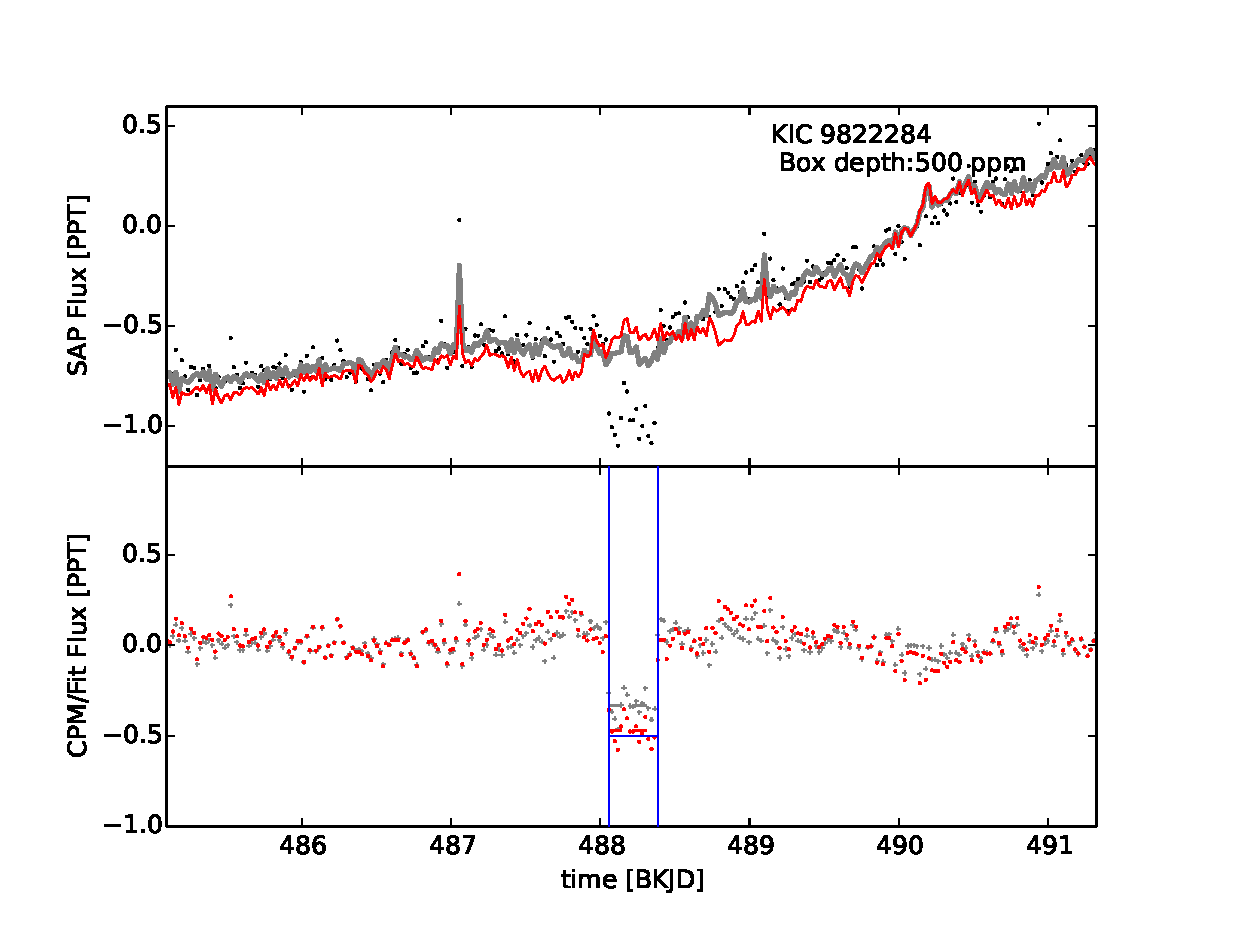
\includegraphics[width=0.32\textwidth]{f4a}
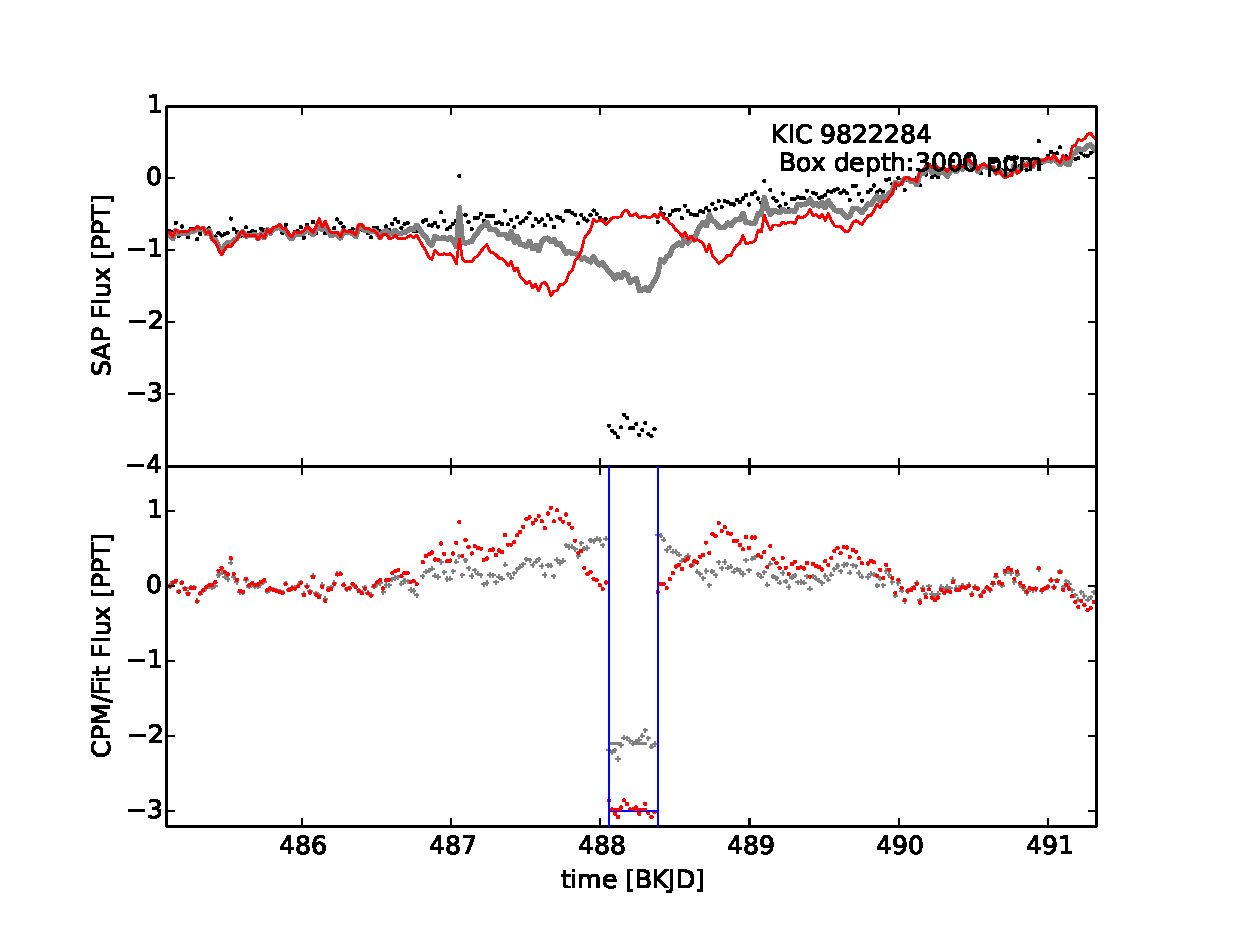
\includegraphics[width=0.32\textwidth]{f4b}
\includegraphics[width=0.32\textwidth]{f4c}
\end{center}
\caption{
  \label{distortion} 
  \name\ preserves transit signals.
  \remove{Fake signal with amplitude 1.0005 is inserted into the single pixel (1, 2) of star KIC 9822284.}\revise{Simply box models with depth from $100 ppm to 1\%$ is injected into the light-curve of star KIC 9822284. Plot (a) and (b) show the results from box model depth to be 500 ppm and 3000 ppm.}
  In the top panel, the black points shows the SAP flux of the pixel with the injected signal, the bold grey line is the fitting of the SAP flux, and the thin red line is the \name\ prediction. 
  In the bottom panel, red points and grey cross represent the \name\ flux and the fit flux, while the signal value is indicated by the horizontal line. 
  \name\ largely preserves the signal while the fitting flux overfit the signal.} 
  \revise{But the \name\ flux is distorted a little around the box model. 
  And there is more distortion with a strong signal.
  Plot (c) shows the signal depth measured in \name\ and fitting flux relative to the true depth with different box model depth. \name\ can consistently preserve more signal than the "ordinary fitting".}
\end{figure}


To give a view on how our method performs, \name\ is applied on several stars with 
known transit signals but different variability and magnitudes as shown in Fig.~\ref{fluxes}. 
From the plots, we can see that \name\ works quite well on these stars, producing the \name\ fluxes 
with low variation and preserving the transit signals.
In addition, \name\ and PDC are compared based on 6 quiet stars 
(non-variable stars, first two rows of Fig.~\ref{fluxes}). 
The results illustrate that for these quiet stars our approach removes 
a major part of the variability present in the PDC light-curves, while preserving the transit signals. 
To provide a quantitative comparison, we ran \name\ on 1000 stars from the whole Kepler input catalog 
(500 chosen randomly from the whole list, and 500 random G-type sun-like stars), 
and estimate the Combined Differential Photometric Precision (CDPP,  \cite{cdpp1} )for \name\ and PDC.  
CDPP is an estimate of the relative precision in a time window, 
indicating the noise level seen by a transit signal with a given duration. 
\revise{In this paper, the CDPP is calculated with 12 bandpass filter using the equations 6-8 in section 3.3 of \citep{cdpp1}. And the CDPP of both PDC and \name\ is estimated with the same algorithm.} 
The duration is typically chosen to be 3, 6, or 12 hours. 
We use the 12-hours CDPP metric, since the transit duration of an earth-like planet is roughly 10 hours. 
Before CDPP is estimated, the variability of the stars are evaluated by median differential variability 
  (MDV, see \cite{basri2013} for details). 
Based on the variability, the 100 most variable stars in the list are removed, 
  since PDC is not designed to remove stellar variability, 
  and we want to compare \name\ and PDC on the close footing.
Fig.~\ref{cdpp} presents our CDPP comparison of \name\ and PDC, 
  \remove{showing that our method (\name) outperforms PDC.}\revise{4 quarters' (quarter 5, 6, 7, 8. Data of quarter 5 are from Kepler data release 21 and other data are from Kepler data release 24---the current version) data are used to show that \name\ has a consistent performance over a whole orbital period of the Kepler photometer (372 days). We also want to emphasis that both \name\ and PDC are presented here does not mean that it is a competition. Since PDC is designed to preserve stellar variability, it is not fair to put \name\ and PDC into competition. The CDPP comparison is made only to give a relative reference how \name\ can perform according to PDC, the Kepler "gold standard"}

\revise{In order to show the overall ability that \name\ have in exoplanet searching, a comparison between \name\ and median filter (a widely used de-trend method) is presented in Fig.~\ref{filter}. This is a more comprehensive comparison, since not only noise level (CDPP) is evaluated,  but how well both methods can retrieve signal from the light curve is also under consideration. In the example, a 200 ppm box model signal is injected into a quiet star KIC 8846139 in quarter 5. With the signal injected light curve,  both methods---median filter and \name\ are applied. As shown in Fig.~\ref{filter}, when  the window size is bigger than 24 hours, \name\ performs better both in terms of CDPP and signal strength. As expected, when the window size gets smaller, CDPP decreases,  while the signal strength retrieved from the light curve also falls off. Although median filter with window size smaller than 24 hours is able to generate cleaner light curves (lower CDPP level) than \name, it largely distorts the signal that we care about. Imagining in an extreme case, light curves generated by a half hour median filter will have zero CDPP, as well as zero signal strength. If we examined the ratio of the signal strength to the CDPP (signal to noise ratio) in this example, it results that \name\ can always have a signal to noise ratio around 8, while the median filter method can only achieve a ratio around 6 in the best circumstance, when window size is 24 hours. Therefore, the example intuitively exhibits that \name\ is able to generate light curves with low noise level as well as preserve the transit signal.}


\begin{figure}[p]
\begin{center}
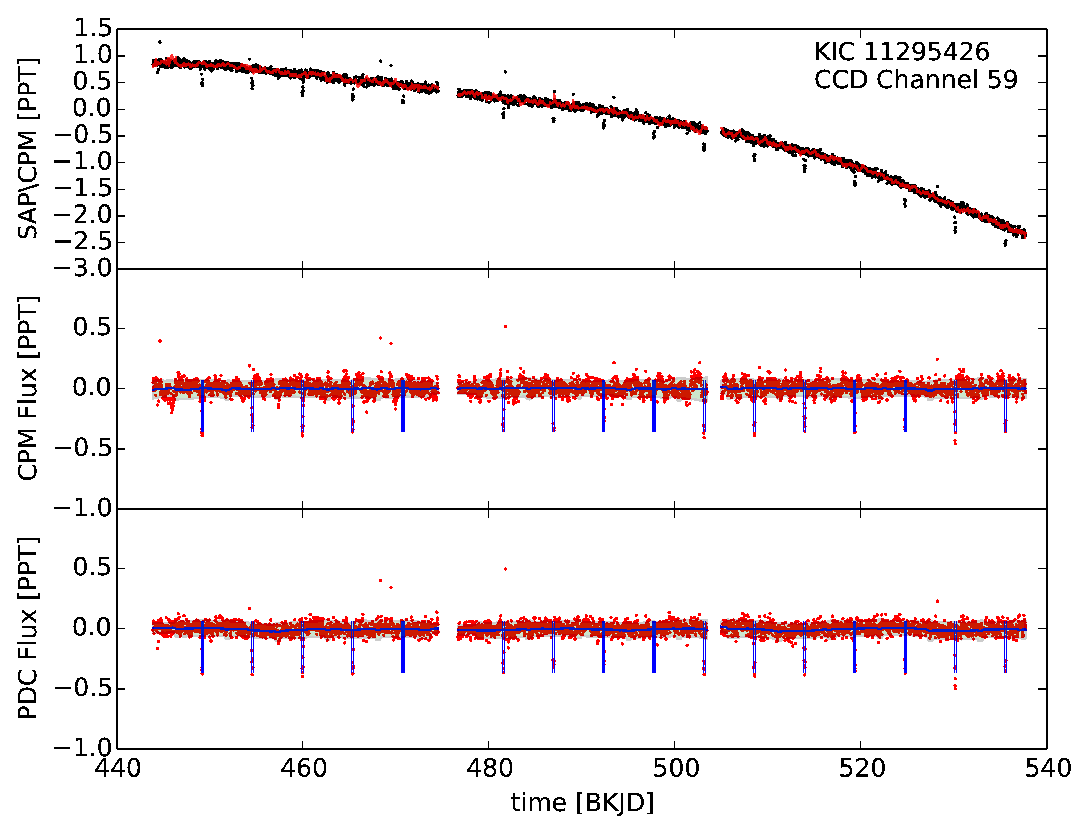
\includegraphics[width=0.32\textwidth]{f5a}
\hfill
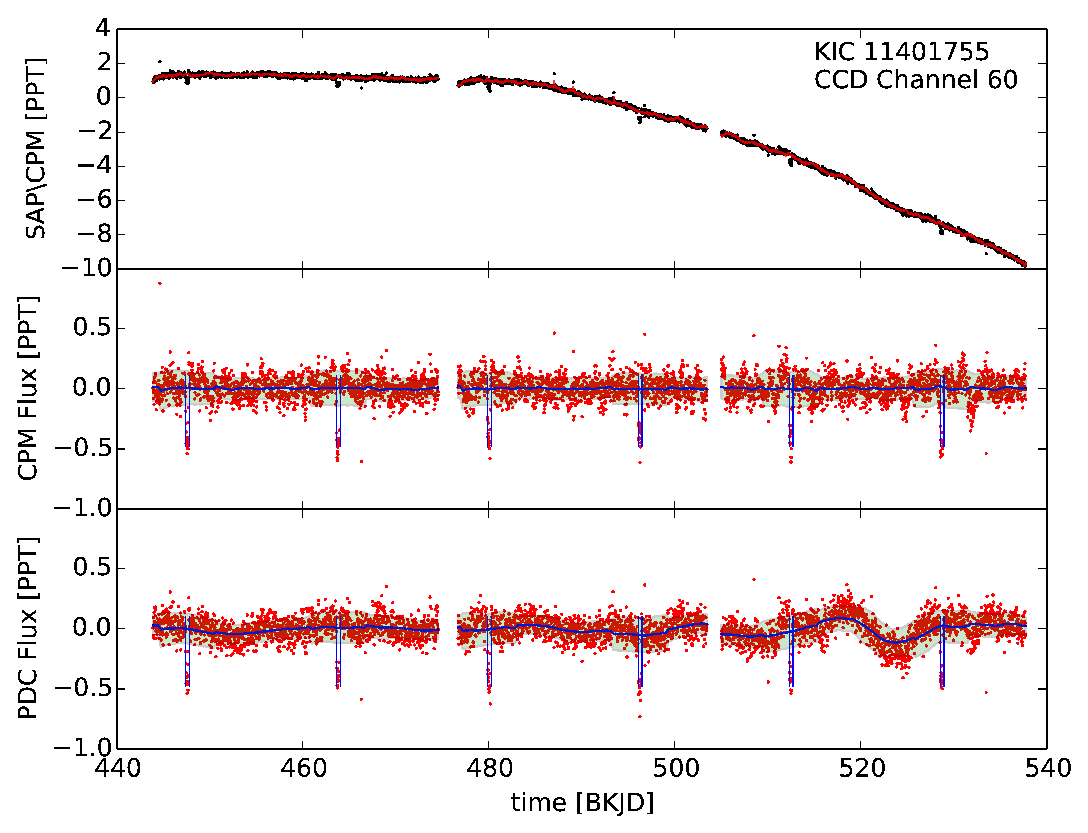
\includegraphics[width=0.32\textwidth]{f5b}
\hfill
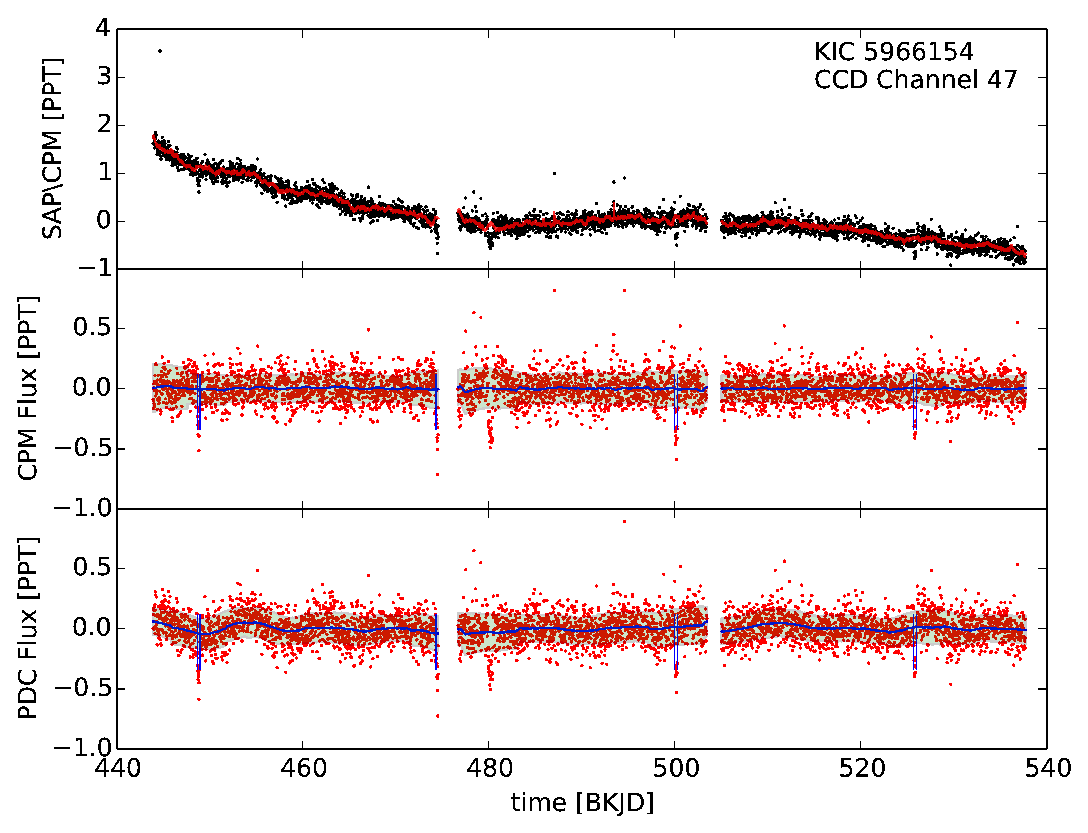
\includegraphics[width=0.32\textwidth]{f5c}


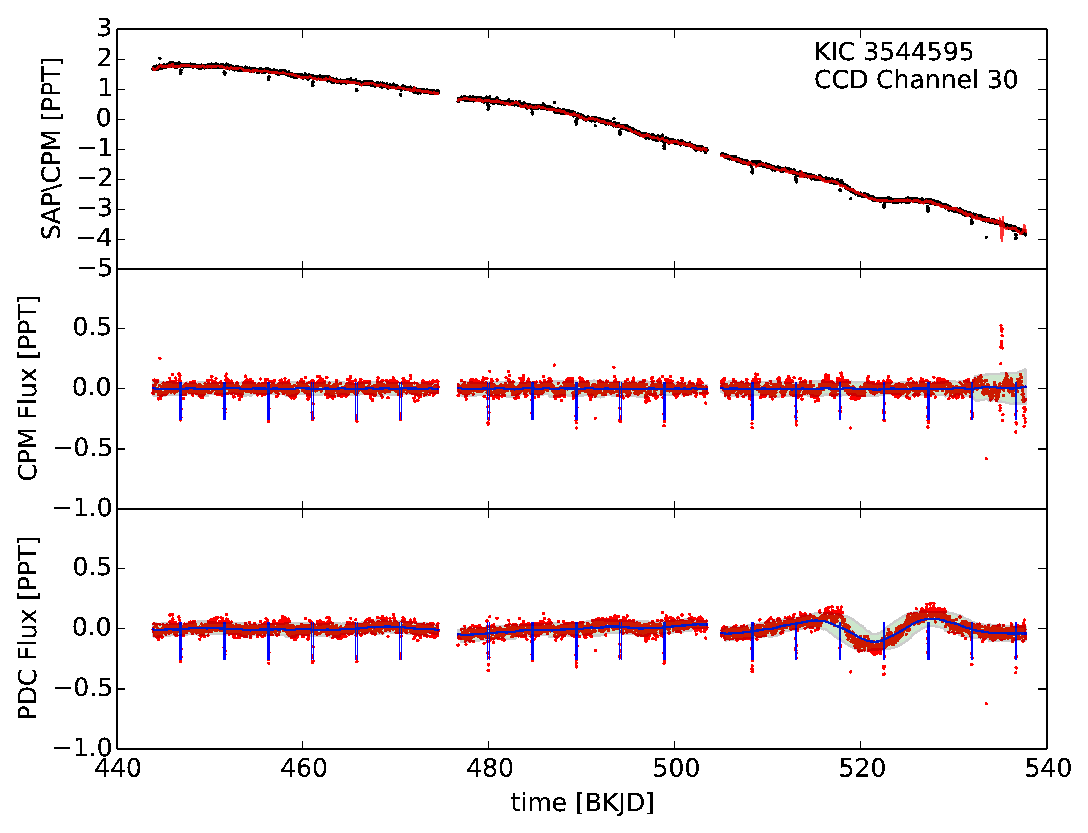
\includegraphics[width=0.32\textwidth]{f5d}
\hfill
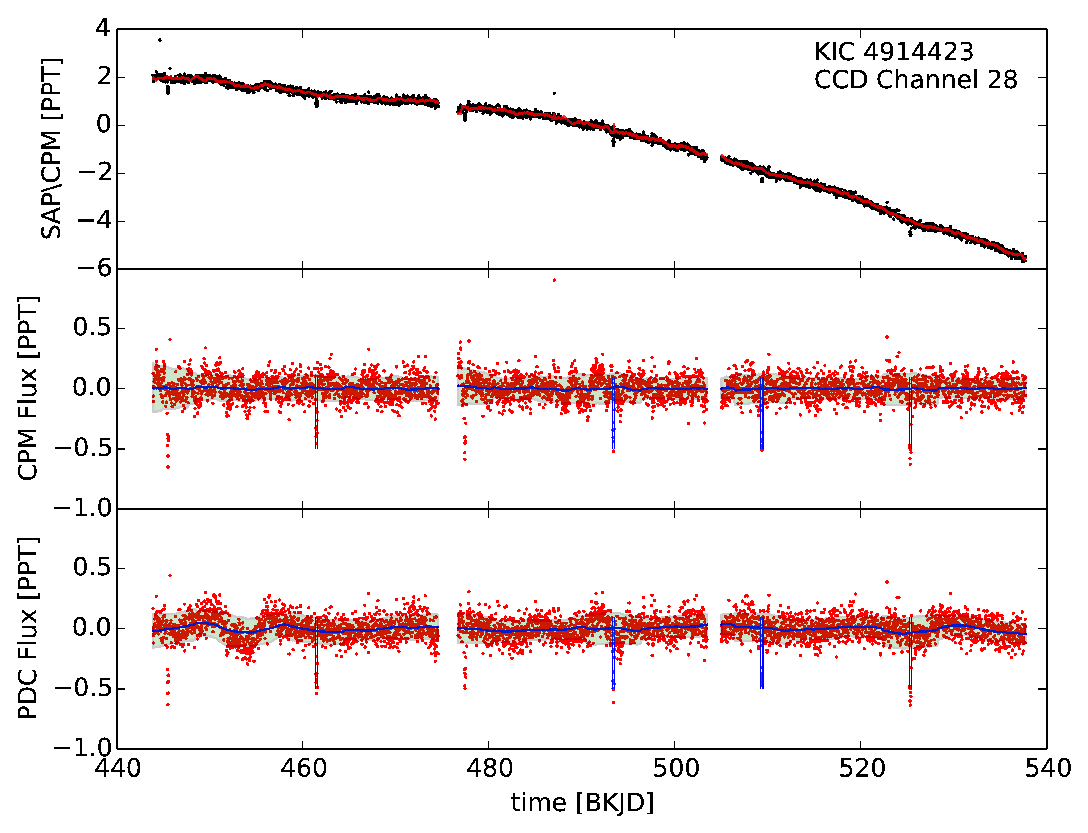
\includegraphics[width=0.32\textwidth]{f5e}
\hfill
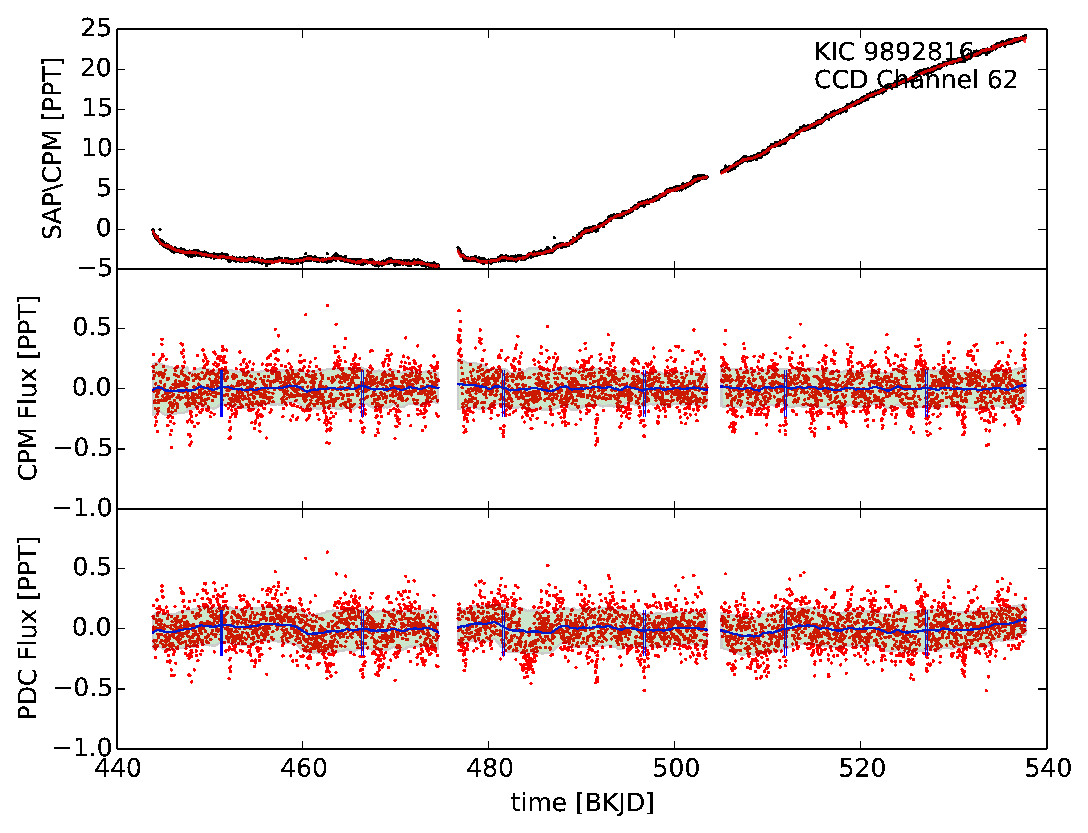
\includegraphics[width=0.32\textwidth]{f5f}


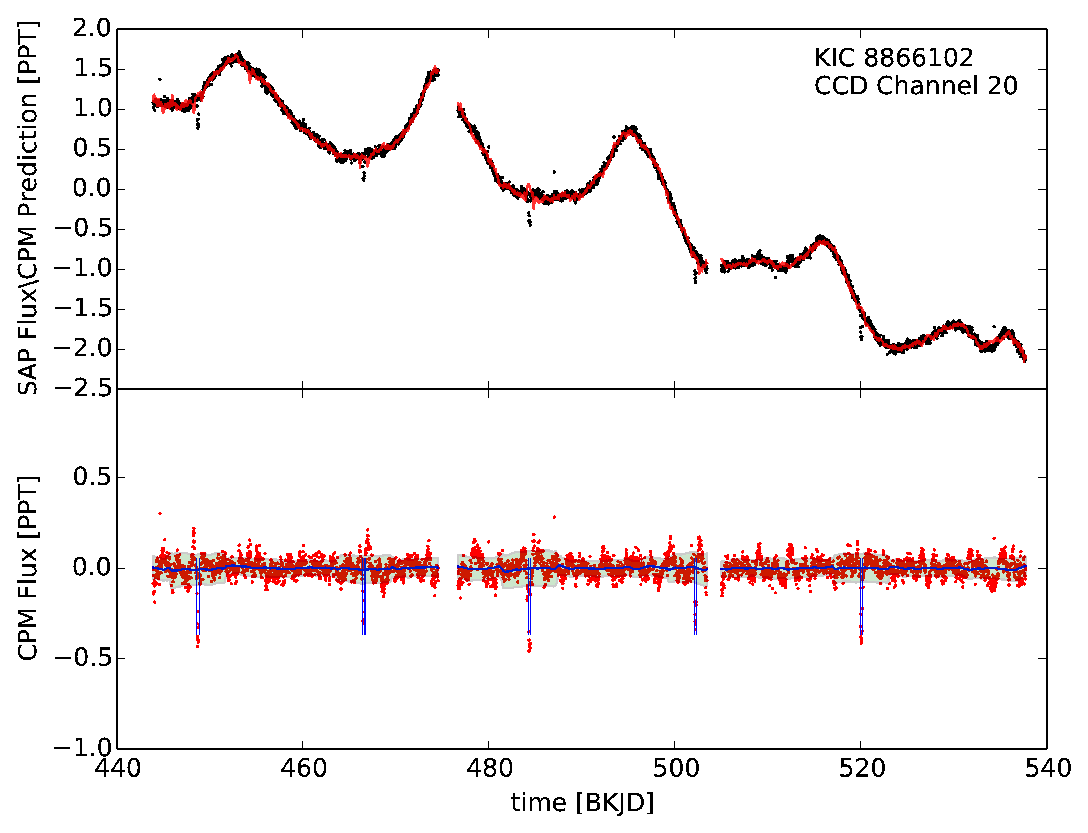
\includegraphics[width=0.32\textwidth]{f5g}
\hfill
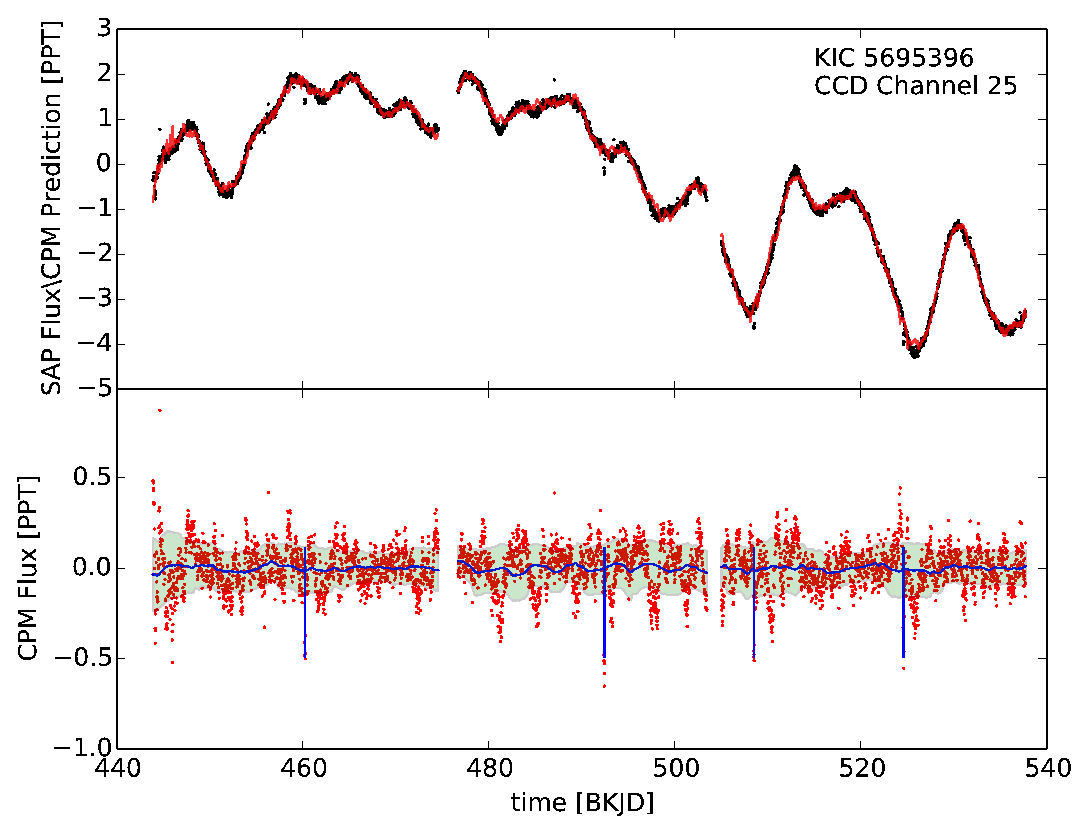
\includegraphics[width=0.32\textwidth]{f5h}
\hfill
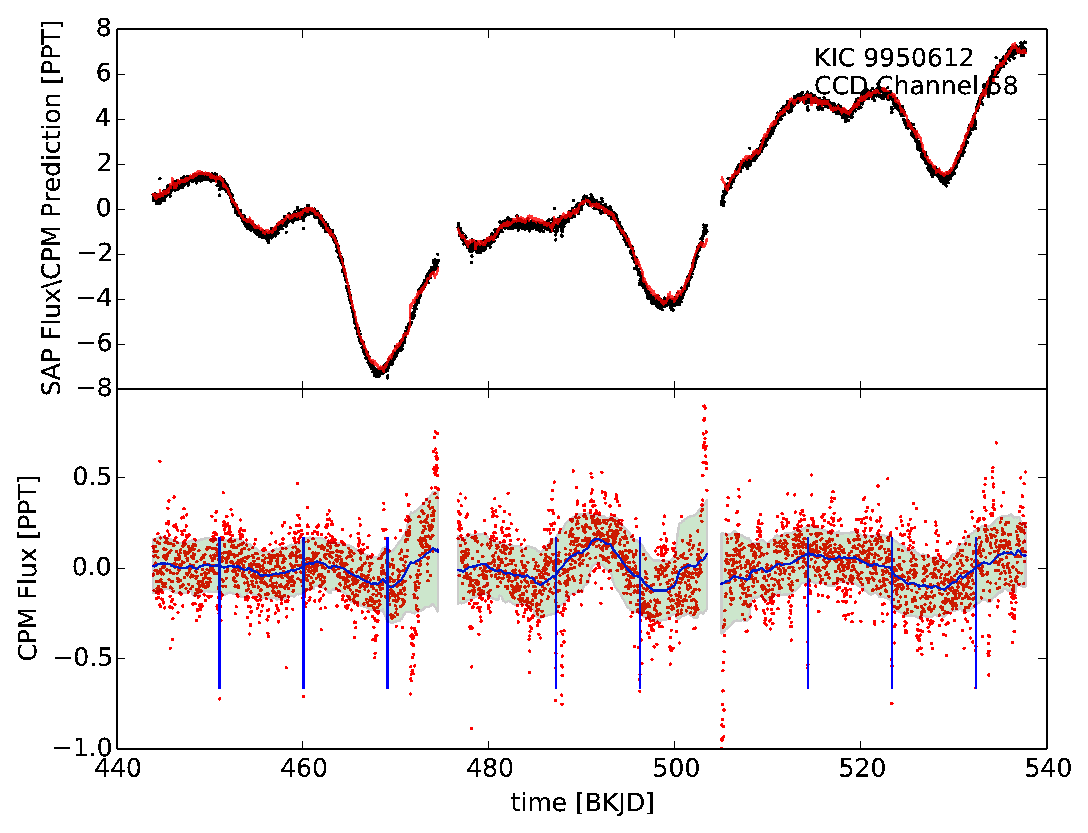
\includegraphics[width=0.32\textwidth]{f5i}


\includegraphics[width=0.32\textwidth]{f5j}
\hfill
\includegraphics[width=0.32\textwidth]{f5k}
\hfill
\includegraphics[width=0.32\textwidth]{f5l}
\end{center}

\caption{
  \label{fluxes} 
  Corrected fluxes using \name, for 12 example stars, 
    spanning the main magnitude (brightness) range encountered. 
  In first column plots, we consider bright stars with magnitude from 9 to 10.5, 
    second cloumn are stars with magnitude from 11 to 12.5,  
    and the third column are faint stars with magnitude above 13. 
  In the first two rows, we present some quiet stars. 
  In all three panels, the top panel shows the SAP flux (black) and the \name\ regression (red), 
    i.e., our prediction of the star from other stars. 
  The middle panel shows the \name\ flux corrected using the regression, and the bottom shows the PDC flux. 
  One can see that the \name\ flux curve preserves the exoplanet transits (little downward spikes), 
    while removing a substantial part of the variability present in the PDC flux. 
  Both the bottom two rows present some variable stars with slow and fast variability. 
  For the variable stars, we did not present the PDC comparison, 
    since the PDC flux try to preserve intrinsic stellar variability.}
\end{figure}

\begin{figure}[p]
\begin{center}
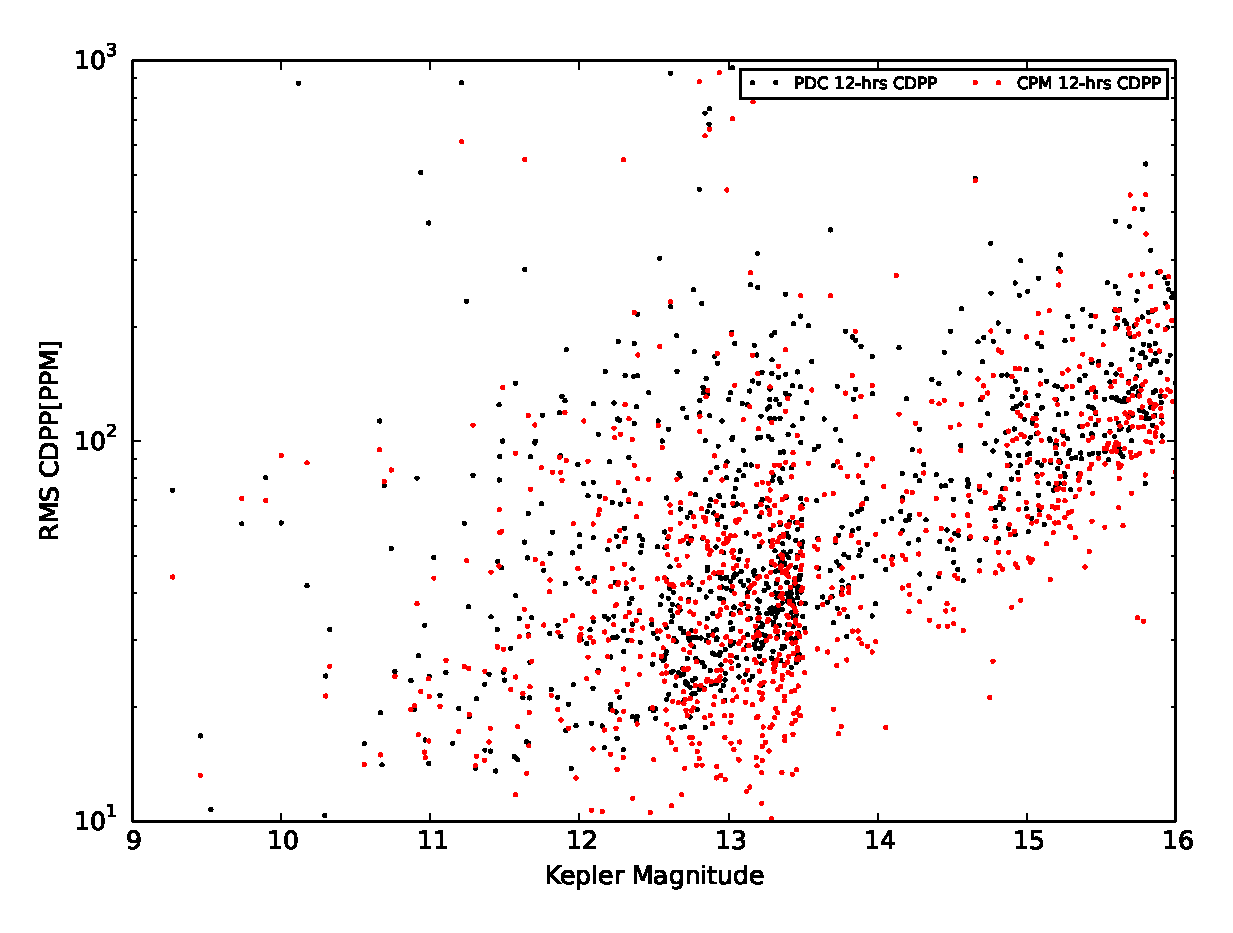
\includegraphics[width=0.32\textwidth]{f6a}
\includegraphics[width=0.32\textwidth]{f6b}
\includegraphics[width=0.32\textwidth]{f6c}

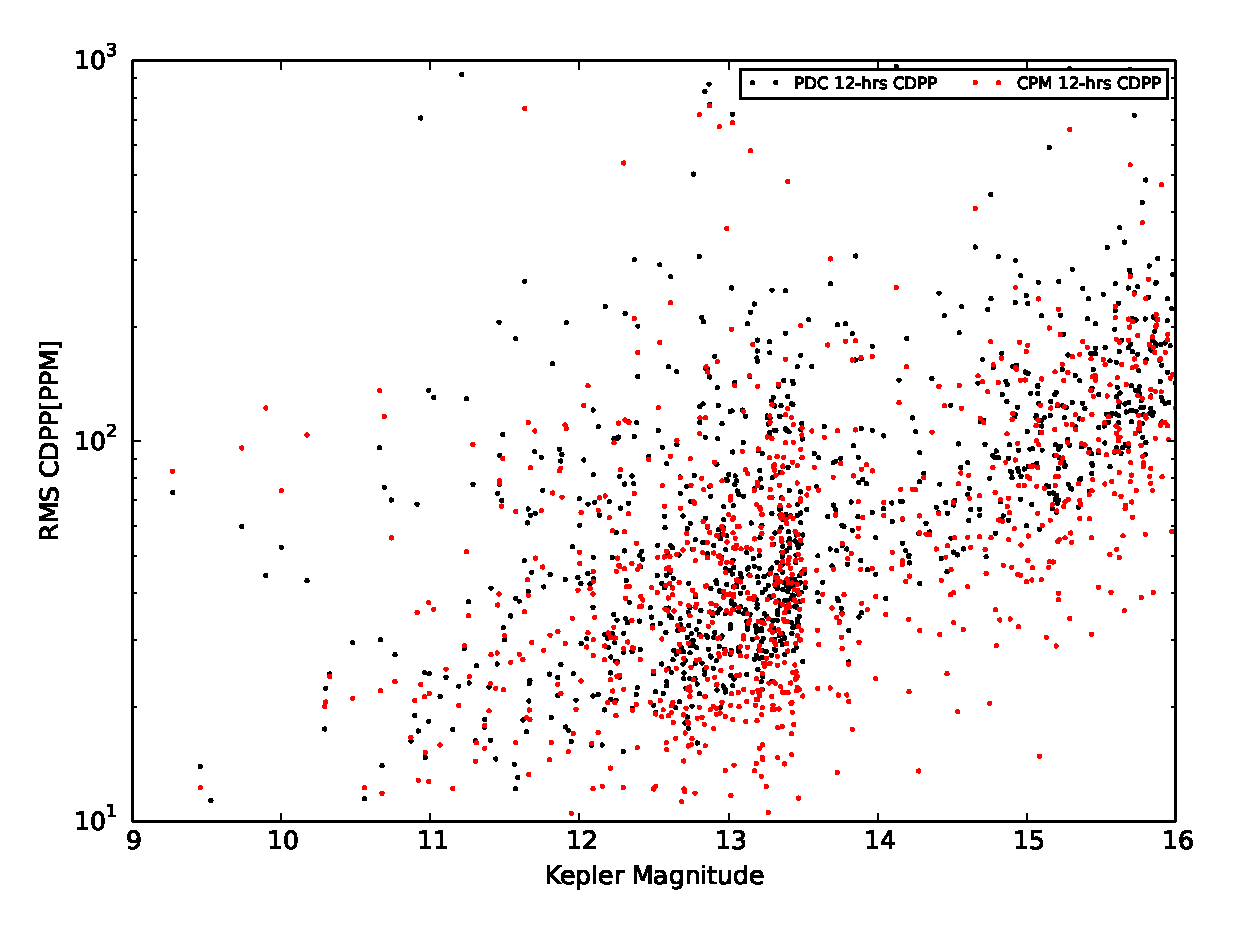
\includegraphics[width=0.32\textwidth]{f6d}
\includegraphics[width=0.32\textwidth]{f6e}
\includegraphics[width=0.32\textwidth]{f6f}

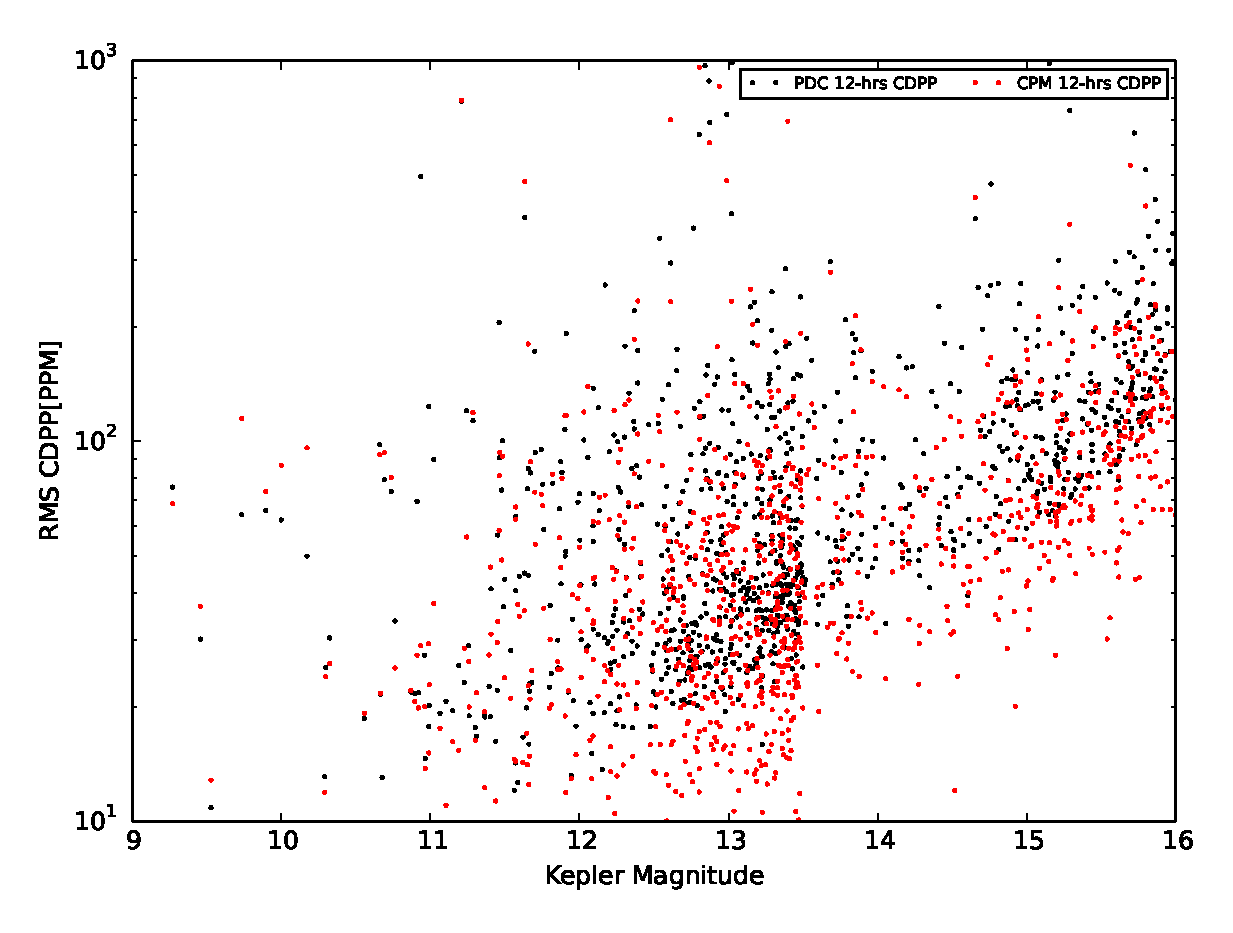
\includegraphics[width=0.32\textwidth]{f6g}
\includegraphics[width=0.32\textwidth]{f6h}
\includegraphics[width=0.32\textwidth]{f6i}

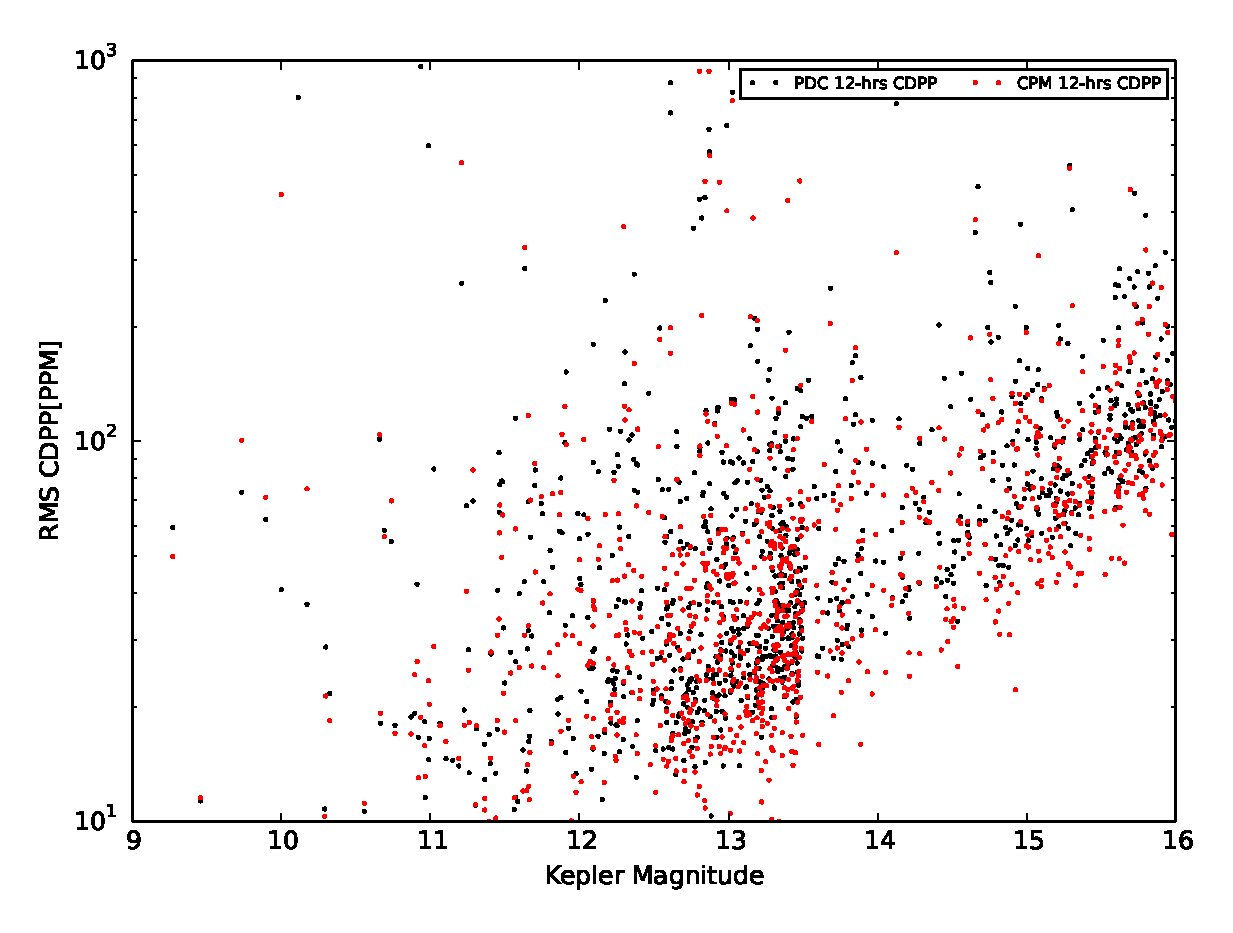
\includegraphics[width=0.32\textwidth]{f6j}
\includegraphics[width=0.32\textwidth]{f6k}
\includegraphics[width=0.32\textwidth]{f6l}
\end{center}
\caption{
  \label{cdpp} 
  Comparison of the proposed method (\name) to the \Kepler\ Pre-search Data Conditioning (PDC) method 
    in terms of Combined Differential Photometric Precision (CDPP).
  \revise{Row 1-4 shows the CDPP estimation throgh quarter 5 to quarter 8. In each row:} 
  Plot (a) shows our performance (red) vs.\ the PDC performance in a scatter plot, as a function of star magnitude 
    (note that larger magnitude means fainter stars, 
    and smaller values of CDPP indicate a higher quality as measured by CDPP.)
  Plot (b) bins the same dataset and shows box plots within each bin, 
    indicating median, top quartile and bottom quartile. 
  The red box corresponds to \name, while the black box refers to PDC. 
  Plot (c), finally, shows a histogram of CDPP values. 
  Note that the red histogram has more mass towards the left, i.e., smaller values of CDPP, 
    indicating that our method \remove{overall outperforms PDC, the Kepler ``gold standard.'' } \revise{process the \Kepler\ light-curve to a lower noise level.}
}
\end{figure}

\begin{figure}[p]
\begin{center}
\includegraphics[width=\textwidth]{f7a}
\end{center}
\caption{
  \label{filter} 
\revise{Comparison of \name\ to the median filter method (based on PDC light curve) with different filter window size. 200 ppm box model signal is injected into the light curve of KIC 8846139 in quarter 5. Both \name\ and median filter method are applied to the light curve after injection. In the first panel, CDPP estimate of the median filtered light curve is plotted as a function of the filter window size (blue dots) and the red dash line indicates the CDPP level of CPM. In the second panel, the signal strength measured from the median filtered light curve is plotted as a function of the filter window size (blue dots), while the red dash line indicates the signal strength retrieved from the \name\ light curve. The grey dash line shows the injected signal strength. Smaller window size reduces the noise level (CDPP) of the median filtered light curve, while distort the signal more. \name\ outperforms median filter in terms of signal to noise ratio.}
}
\end{figure}

\section{Discussion}
We have presented a simple yet highly effective method---the \name\ that works in pixel-level 
  based on the causal structure of the \Kepler\ data to calibrate the \Kepler\ light-curves, 
  which is intended to search exoplanets.
In \name, systematics and stellar variabilities are removed by
  either fitting with other stars' light-curves or auto-regressive components,
  while transit signals can still be perfectly preserved by train-and-test framework.
Low variable clean light-curves can be produced by \name\,  
  which is ideal for transit planet searching. 
The CDPP noise level estimation is also presented in the paper to show the performance of \name. 

Apart from the \name, as mentioned in the beginning of the paper, 
  there exist several other methods that are effective in de-trending the light-curve.
Methods like median filter are quite successful in smoothing all the unwanted features 
  either from spacecraft or intrinsic stellar variability, 
  but the problem is that this kind of methods filter everything in the data including the transit signal. 
This is not a big deal for searching giant planets, since the signal is quite strong. 
However, 
  when it comes to earth-like planets (only about \remove{20 ppm}\revise{$\backsim 100\ ppm$} transit signal around a sun-like star),
  \remove{any reduction or distortion of the signal is unacceptable.}
  \revise{preventing transit signal from reduction or distortion is important.} 
In comparison, in order to achieve higher precision for earth-like planet searching, 
  \name\  not only exploits the causal structure of the \Kepler\ data,
  but also apply effective approaches (strong regularization and train-and-test framework)
  to avoid over-fitting the transit signal.
There also exists more sophisticated method like PDC.
As mentioned earlier in this paper, 
  \name\ is very similar to PDC, 
  in that they both make use of the correlation between light-curves,
  which is assumed to be caused by the spacecraft effects (or systematics).
\remove{However, in section 4, we show that \name\ performs better than PDC, 
  in that it has a overall low noise level (CDPP).
We think the outperformance mainly caused by two factor.}
\revise{However, the main difference between \name\ and PDC lays on two factor.}
One is that \name\ calibrates every single pixel separately, 
  while PDC works in the photometry level.
It is no doubt that pixel-level modelling enables \name\ capture more variability, such as 
variations in the centroids and point-spread function from spacecraft pointing, roll, and temperature.
The other reason is that,  
  in PDC,  only leading eight principal components of some relative light-curves are used.
Although restricting the number of components can prevent over-fitting, we think with this limited number of components, 
  it is insufficient to capture all the variabilities in the light-curve.
In \name\, hundreds of stars' light-curves (or thousands of pixels) are used 
  to capture relatively complete information of the variabilities, 
  while strong regularization and train-and-test framework are applied to prevent over-fitting.
Although we present the comparison between \name\ and PDC, 
  we still want to emphasis that PDC is a method intended to preserve stellar variabilities, 
  while the \name\ is optimized for exoplanet searching. 
The comparison is only based on our objective (search for earth-like planet), 
  and should not be regard as standard of a best model for \Kepler\ data.
  
However, apart from the outstanding performance in calibrating the data, the \name\ still has several issues. 
Based on our assumption of the causal structure of the \Kepler\ data, 
  if we turn off the auto-regressive components and keep the predictors from other stars working in the \name, 
  we should be able to still remove the systematics while preserve the intrinsic stellar variability, 
  since there is no reason that these independent stars can be used to predict the stellar variability of the target star.
However, in fact, we can not preserve the stellar variability just by turning off the auto-regressive components. 
One possible reason can be that, since our model is so flexible (thousands of parameters), 
  in principle it can fit any functions. 
In this sense, 
  we should run cross-validation with the auto-regressive components turned off 
  and to find out how many pixels from other stars we need to just remove systematics 
  while preserve stellar variability, 
  but in fact we do not have a good criterion to check how well we preserve stellar variability in cross-validation 
  because we do not have enough knowledge of the true stellar variability. 
Thus for the time being, we just focus on producing well-calibrated light-curves for searching exoplanets, 
  but in long term, we are looking forward to find a method to preserve the stellar variability.

Another issue of the \name\ is that when there are strong transit signals in the light-curve,  
  one can find distortion around these signals.
We think this problem is caused by the train-and-test framework.
Train-and-test framework is applied in the \name\ to preserve the transit signals, 
  in which data points in a certain excluded window are separated from the model.
However, for data points half-window size away from the transit signals, 
  the prediction of these points in \name\ is largely influenced by the strong transit signal.
That is,  these points are predicted to be a little bit smaller than they should be, 
  since transit signal (negative points away from the continuum) makes the model think
  there is a decreasing trend in this region.
This window edge effect is a trade-off of the train-and-test framework that is crucial for \name,
 and can not be solved in the scope of \name.

One possible way to solve this kind of edge effect 
  but still preserve the transit signals is to do the simultaneous fitting 
  for both systematics and transit signal together, 
  like what have been done in \cite{dfm}. 
That is,  
  instead of only modelling the systematics 
  and then subtracting it from the raw data to produce some de-trended light-curves,
  a comprehensive model for all components in the data (systematics, stellar variabilities and transits)  can be made. In this kind of model, there is no need for train-and-test framework,
  since all transit signals have already been modelled 
  and no de-trended light-curve will be produced. Planets will be found directly in the model itself. 

\revise{Another issue or improvement that can be considered for \name\ is the predictor selection algorithm. 
In \name\, a simple selection policy is applied, in which closest stars in magnitude on the same CCD channel are selected. This algorithm might be reasonable, since intuitively, the response function of CCD might be similar for stars with similar brightness. 
However, Kepler is a complicated system. Systematics like rolling bands may affect only some of the stars. Chances are that "bad predictors" may be included into the set of predictor stars to distort the \name\ prediction or \name\ might miss some of the "good predictors", in which case, it can not capture some of the systematics signature. Although we also want to mention that in \name\, a huge set of predictors (4000 pixels from other stars) are used, which somehow ensures the model perform well in general, it still remains an unsolved issue for \name.
In this paper, we did not purse the optimized selection algorithm, because we want to make the model as simple as possible. But in order to get an optimized performance for \name, how to select and rank the predictor stars is an important and unavoidable issue.}

\revise{As we have mentioned before in this paper,  since \name\ needs to make prediction for every data points in the light curve, it is quite time-cosuming to process the complete Kepler data set with \name. Here we presents an \name\ runtime estimation based on our experience.  For a light curve of duration three months (one quarter), \name\ took about 7 hours on a single core (Ivy Bridge x86 64 3.0GHz).}

However, despite all the problems mentioned in the \name,
  we expect that data-driven model like our method will enable astronomical discoveries 
  at higher sensitivity on the existing \Kepler\ data as well as on future missions.  
As we know, \Kepler\ \project{K2} \citep{k2} data are suffering from the broken-down of reaction wheels, 
  which makes the \remove{satellite}\revise{space craft} hard to control and introduce significant systematics. 
Flexible data-driven model \citep{dfm} has already shown the power on the \project{K2} data 
  and find new planets.
Moreover, in 2017, NASA is planning the launch of another space telescope---
  \project{TESS} (Transiting Exoplanet Survey \remove{satellite}\revise{space craft}, \cite{tess}), 
  which will perform an all-sky survey for small (earth-like) planets of nearby M stars. 
  We think our method can be simply extended for these project to help achieving higher precession and more scientific results. 


\acknowledgements
It is a pleasure to thank the whole \Kepler\ Team
  for designing, delivering, and operating a great facility,
  and for making all of the data public, in all its rawest forms, through the MAST interface.
We are also pleased to thank
  Ruth~Angus (Oxford),
  Tom~Barclay (Ames),
  Bekki~Dawson (Berkeley),
  Rob~Fergus (NYU),
  Stefan~Harmeling (Dusseldorf),
  Michael~Hirsch (UCL),
  Dustin~Lang (CMU),
  Benjamin~T.~Montet (Caltech),
  David~Schiminovich (Columbia),
  and
  Jake Vanderplas (UW)
for valuable discussions, input, encouragement, and advice.
This project was partially supported by
  NSF grant IIS-1124794,
  NASA grant NNX12AI50G.
  the Moore Foundation,
  and
  the Sloan Foundation.
This research made use of the NASA Astrophysics Data System.

\clearpage
\bibliography{cpm}
%% This file is part of the causal-kepler project
% Copyright 2013, 2014 the authors.

%

\documentclass[12pt, preprint]{aastex}

\newcommand{\notenglish}[1]{\textit{#1}}
\newcommand{\sic}{\notenglish{sic}}
\newcommand{\project}[1]{\textsl{#1}}
\newcommand{\Kepler}{\project{Kepler}}
\newcommand{\name}{CPM}
\newcommand{\set}[1]{\mathcal{#1}}
\newcommand{\given}{\,|\,}
\newcommand{\todo}[1]{\textbf{#1}}

\begin{document}

\title{%
  Self-calibration of time-domain imaging for exoplanet science, informed by causal structure%
  \\ or \\
  A data-driven, pixel-level model to improve the precision of \Kepler\ photometry%
  \\ or \\
  Exploiting causal structure to create a data-driven self-calibration of \Kepler\ imaging%
}
\author{%
  Dun~Wang\altaffilmark{\ref{CCPP}},
  Dan~Foreman-Mackey\altaffilmark{\ref{CCPP}},
  David~W.~Hogg\altaffilmark{\ref{CCPP},\ref{CDS},\ref{MPIA},\ref{email}},
  Bernhard~Sch\"olkopf\altaffilmark{\ref{MPIIS}},
  others%
}
\newcounter{address}
\setcounter{address}{1}
\altaffiltext{\theaddress}{\stepcounter{address}\label{CCPP}%
  Center for Cosmology and Particle Physics, Department of Physics, New York University}
\altaffiltext{\theaddress}{\stepcounter{address}\label{CDS}%
  Center for Data Science, New York University}
\altaffiltext{\theaddress}{\stepcounter{address}\label{MPIA}%
  Max-Planck-Institut f\"ur Astronomie, Heidelberg, Germany}
\altaffiltext{\theaddress}{\stepcounter{address}\label{email}%
  To whom correspondence should be addressed; \texttt{<david.hogg@nyu.edu>}.}
%% \altaffiltext{\theaddress}{\stepcounter{address}\label{Ames}%
%%   NASA Ames Research Center}
%% \altaffiltext{\theaddress}{\stepcounter{address}\label{Courant}%
%%   Courant Institute of Mathematical Sciences, New York University}
\altaffiltext{\theaddress}{\stepcounter{address}\label{MPIIS}%
  Max-Planck-Institut f\"ur Intelligente Systeme, T\"ubingen}
%% \altaffiltext{\theaddress}{\stepcounter{address}\label{Oxford}%
%%   Department of Physics, Oxford University}
%% \altaffiltext{\theaddress}{\stepcounter{address}\label{CfA}%
%%   Harvard--Smithsonian Center for Astrophysics}
%% \altaffiltext{\theaddress}{\stepcounter{address}\label{UCL}%
%%   Department of Physics and Astronomy, University College London}
%% \altaffiltext{\theaddress}{\stepcounter{address}\label{CMU}%
%%   McWilliams Center for Cosmology, Carnegie Mellon University}
%% \altaffiltext{\theaddress}{\stepcounter{address}\label{Caltech}%
%%   Department of Astronomy, California Institute of Technology}
%% \altaffiltext{\theaddress}{\stepcounter{address}\label{Columbia}%
%%   Department of Astronomy, Columbia University}

\begin{abstract}
The precision of \Kepler\ photometry for exoplanet science---the most
precise photometric measurements of stars ever made---appears to be
limited by unknown or untracked variations in spacecraft pointing and
temperature, and unmodeled stellar variability.
Here we present \name,
  a data-driven model of these variations in \Kepler\ data (or really of their impact on the photometry).
Importantly (and uniquely),
  \name\ works at the pixel level (not the photometric measurement level);
  it can capture more fine-grained information about the variation of the spacecraft
  (especially regarding pointing and point-spread function)
  than is available in the pixel-summed photometry.
\name\ is extreme in that it has enormous flexibility and it only uses data (and meta-data) to predict data:
\name\ provides a prediction for each readout pixel built from a linear combination of the readouts
  from very large numbers of nearby pixels (plus some spacecraft information);
  the choice of nearby pixels is guided by ideas from causal inference.
\name\ avoids over-fitting by employing a train-and-test formalism
  designed to ensure that transit-like photometric events and short-timescale stellar variability
  cannot be captured or distorted by the model;
  it is designed to remove spacecraft-induced variability but not intrinsic stellar variability.
We show that \name\ outperforms the \Kepler\ Presearch (\sic) Data Conditioning method on a set of example stars.
We release open-source code that provides \name\ output for any star in the existing \Kepler\ Archive,
  and we discuss applications for other missions,
  including any possible \Kepler\ two-wheel mission.
\end{abstract}

\section{Ultra-precise photometry}

The photometric measurements of stars made by the \Kepler\ Satellite are precise enough
  to permit discovery of exoplanet transits with depths smaller than $10^{-4}$.
This precision results from great spacecraft stability,
  supplemented by various methods for removing small residual spacecraft-induced and stellar-variability trends in the brightnesses,
  either filtering the data (with things like median filters; \todo{citations})
  or fitting the data with flexible models (like polynomials or splines or Gaussian Processes; \todo{citations}).
When employed in the service of exoplanet search and characterization,
  these methods are usually agnostic about whether photometric variations originate in the spacecraft or in the star itself;
  that is, they obliterate intrinsic stellar variability along with spacecraft issues.

In general, there are many reasons for apparent photometric variability in a \Kepler\ source.
There is intrinsic stellar variability,
  which is of interest to some and a nuisance to others.
There is also variability of overlapping fainter stars;
  that is, confusion noise combined with variability of the confusing sources.
There are small changes in spacecraft pointing,
  which leads to slightly different illumination of the focal-plane pixels,
  and thus different sensitivity to errors (problems) in the device flat-field or sensitivity map.
There are also \emph{intra-pixel} sensitivity variations that can contribute (\todo{cite white paper; Spitzer results}).
There are small changes in spacecraft temperature,
  which lead to point-spread function (PSF) and differential (across the focal plane) pointing changes.
These also lead to changes in pixel and intra-pixel illumination.
Stellar proper motion, geometric parallaxes, and differential stellar aberration as the spacecraft orbits all do more of the same.
There is electronic cross-talk between detectors and charge-transfer inefficiency;
  these can effectively transfer variability from one source to another.
There are additional electronics effects like ``rolling bands'' that put additional features into lightcurves.
There are also probably changes to the detector sensitivity with temperature and time,
  possibly illimunation-history effects,
  and possibly sources of variability not yet considered.
The remarkable thing about \Kepler\ is that it is trying to measure stars at a level of precision
  much higher than ever previously attempted;
  new effects really \emph{must} appear at some point.
In \figurename~\ref{fig:pixelpatch}, we show the pixel-level variability in the \Kepler\ data
  near one bright star that shows minimal intrinsic variability;
  this figure highlights the spacecraft-induced effects.

We propose and advise dealing with these variations in \Kepler\ light-curves by \emph{modeling} them.
In this context, a model is (at least) a parameterized function that can predict data, given parameter settings,
  and an objective function that can be optimized or sampled to choose or set those parameters.
Ideally the objective function is probabilistic, or has a probabilistic justification,
  as with a likelihood or a posterior pdf.
The model can be a physical model (of the spacecraft PSF, pointing, temperature, and so on)
  or it can be a flexible, effective model that has no direct interpretation in terms of physical spacecraft parameters.
In principle a physical model will do a better job,
  because it necessarily embodies more prior information,
  but it requires research and intuition about dominant effects,
  and this research and intuition is often wrong or incomplete.
The model we propose here is in the non-physical, effective category.
The \Kepler\ community is familiar with these kinds of models;
  to our knowledge, \emph{all} successful light-curve ``de-trending'' methods
  are flexible, effective models.

One such method---one that is designed to describe or model spacecraft-induced problems
  but \emph{not} interfere with measurements of stellar variability---%
  is the \Kepler\ Presearch (\sic) Data Conditioning (PDC) method (\todo{citation}).
The PDC ``de-trends'' the \Kepler\ lightcurves by fitting them with a small set of basis lightcurves
  generated from a principal components analysis (PCA) of filtered lightcurves.
That is, it uses data to predict data,
  regularizing the fit (and avoiding over-fitting) by filtering and restricting the dimensionality (through PCA).
The method proposed here, \name, is very similar in spirit to the PDC.
The main differences are
  (1)~that \name\ works in the pixel domain, not the lightcurve domain, so it has access to more fine-grained information,
  (2)~that \name\ has far more freedom (far more parameters) than the PDC
  but it strictly avoids over-fitting the lightcurves on exoplanet-transit time-scales
  through strong regularization and a train-and-test framework, and
  (3)~that when \name\ fits a star, there is no possibility of any contribution of the star itself to the fit basis vectors.
The two methods (\name\ and PDC) are similar however,
  in that they both make the assumption that whatever spacecraft effects are imprinting variability on a stellar lightcurve
  must also be imprinting similar or related variability on other lightcurves.
They also assume that the relationships can be captured with linear models.
By going to the pixel level (unlike the PDC, which works at the photometry level),
  \name\ makes it easier for the model to capture variability
  that is coming through variations in the centroids and point-spread function
  from spacecraft pointing, roll, and temperature.

Before we start, a few reminders about the \Kepler\ data are in order:
The satellite always observes precisely the same field, at fixed pointing (as closely as possible).
Only a few percent of the 80 million pixels in the focal plane are telemetered down
  to Earth from each 30-min exposure;
  the telemetered pixels are associated with \Kepler\ target stars chosen for study by the \Kepler\ Team.
The satellite is rolled by 90~deg every 90-ish days (to satisfy Solar-Angle constraints).
The focal plane contains many CCDs;
  this plus the 90-deg rotations means that each star is at a particular location
  on a particular CCD for 90-ish-day contiguous periods of time.
The PSF varies strongly across the field and is badly sampled.
The stars span a huge range in brightness;
  some of \Kepler's most important targets even saturate the device and bleed charge.
The stellar photometry returned by the \Kepler\ SAP and PDC pipelines is based on
  straight, \emph{unweighted} sums of pixels in small patches centered on the stellar centroid.
We will return to this latter point at the end;
  this kind of photometry cannot be optimal;
  it must be possible to do a better job with the photometric measurements.
That's beyond the scope of this project but a place for a valuable intervention on the \Kepler\ data.

The scope of this project is an intervention---\name---that makes the \Kepler\ photometry more precise.
We describe the method and deliver all the relevant code in a public, open-source repository.
We also provide an interface to the \Kepler\ data that delivers improved ``\name\ photometry''
  for every \Kepler\ target.

\section{Data-driven models}

The first general idea about data-driven modeling of the kind used here
  is that each data point or data source is going to be 
  \emph{predicted} with or using a parameterized mathematical function of \emph{other data}.
That is, given a choice of some \emph{target} \Kepler\ data,
  we are going to find parameters of a function that takes as input some of the other \Kepler\ data,
  and provides as output predictions of the target data.
The simplest models are \emph{linear models},
  in which predictions for the target data are built from linear combinations of the other data,
  and in which the objective functions are quadratic in the prediction residual.
Examples of quadratic objective functions include Gaussian likelihoods, mean-squared-error, and chi-square statistics.
These models are simple,
  not just because they are easy to express and compute,
  but because optimization is convex:
There is only one optimum for the objective function.

The point of these models is to be \emph{flexible},
  so the usual approach is to make the input data set very large,
  and the number of parameters large,
  often as large as---or larger than---the target data available.
Such fits require \emph{regularization} to break degeneracies
  and control ill-constrained parameters.
These regularizations do for optimizations what priors do for posterior probability inferences;
  they express the desired behavior of the fit in the absence of data
  or along directions in parameter space in which the data are not constraining.
General regularizations or priors will break the convexity of linear models;
  if convexity is to be maintained, these regularizations also have to be quadratic,
  or else one of a small number of other known forms (one of which is L1-regularization).
Given these considerations, it makes sense to try to build our pixel-level model
  using a linear model with a quadratic objective function and a quadratic regularization;
  this is what \name\ will be.

The second general idea about data-driven modeling is the investigator's beliefs
  about the causal processes that generate the data
  are crucial in restricting the kinds of data that can be used as input to the model.
That is, different assumptions about the physical properties of the data
  and the data-taking system
  lead to different structures for the data-driven model.
For example, in the case of \Kepler\ data,
  if we believe that different stars in the \Kepler\ field vary independently
  (that is, are not physically synchronized in any way),
  then the only reason that one star might show variability that is strongly \emph{predictive}
  (useful for prediction) of another star's variability
  is that both stars are being observed by the same device or spacecraft.
That is, one star's pixels can be used to predict another star's pixels
  inasmuch as spacecraft issues imprint on both stars in related ways;
  they share a common cause.
For another example, if we think the spacecraft is being affected by
  processes that take place over time-scales longer than a single read-out
  (for example, thermal processes),
  then it would be sensible to model the data at time $t$ using not just simultaneous data,
  but also data from a range of times around $t$.
For another example, if an investigator doesn't care about preserving stellar variability,
  and just wants to detect exoplanet transits (say),
  pixels from the target star can be used to predict pixels from the target star,
  provided they are at large-enough time lags that they don't overlap (in time)
  the signals of interest.
That is, if the model is designed to fit not just spacecraft variability
  but also intrinsic stellar variability,
  the predictive model will be permitted to use as input pixels that \emph{do} overlap the target star.
In what follows, we are only going to use input data that do not overlap that target star pixels.
These models ought to remove spacecraft variability but not intrinsic stellar variability.

The third general idea is that we need to control for over-fitting.
That is, once you have a flexible-enough model you can in principle fit \emph{anything},
  whether it was caused by the spacecraft, intrinsic stellar variability, or a transiting exoplanet.
How do you prevent a very flexible model from taking small noise-induced fluctuations in all the input data
  and carefully combining them linearly into detailed models for every nook and cranny in the target data?
In most projects in astrophysics, over-fitting is controlled for by limiting model freedom.
The model is restricted in the number of parameters
  (as in ``you can't have more parameters than data points'')
  or by limiting the dimensionality
  (as in principal components analysis)
  or by applying strong priors
  (as with smoothness priors, that effectively reduce freedom without explicitly reducing the number of parameters).
In each case, the restriction on model freedom is controlled by some \emph{hyper-parameter}
  (such as the number of inputs, or number of principal components, or the strength of the smoothness prior).
The hyper-parameters can be set or tested with tools like cross-validation,
  the fully marginalized likelihood (Bayes factor or evidence),
  chi-squared statistical criteria,
  or intuition or heuristics.
Here we take a different and more general approach, which is to use a train-and-test framework.

In this framework, the data used to \emph{train} the model%
  ---meaning set the values of the parameters of the model---%
  are disjoint from the \emph{test} data
  ---meaning the data that are being predicted (the target data).
Because we are extremely concerned with detecting Earth-analog exoplanet transits,
  which take about ten hours,
  we adopt an extreme version of the train-and-test framework,
  in which the training data are always separated from the test data by at least ten hours.
That is, when we are using the model to predict a particular pixel in the target data taken at time $t$,
  we use parameters obtained by an optimization that makes use of only data
  that comes either at times prior to $t-\Delta t$ or after $t+\Delta t$,
  where $\Delta t$ is a tunable parameter but which we will set to roughly $12$~h.
This ensures that no information about any exoplanet transit itself
  can be entering into the prediction of the pixels contributing to the stellar photometry.
In general, if there is a scientific goal of preserving intrinsic stellar variability,
  or transit signals,
  on time-scales of $\tau$,
  the parameter optimization ought to be based on training data taken with a time-exclusion zone of half-width $\Delta t > \tau$.

In addition, each training data set within which we set the parameters (by optimization) has a finite total time extent $t_{\max}\approx 90$\,d.
The train-and-test framework, which includes data out to time $t_{\max}$ but excludes data within $\Delta t$ of the test data,
  effectively assumes that the signals worth preserving have time-scales less than $\Delta t$ but don't recur on time-scales
  shorter than $t_{\max}$.
Those assumptions are good for our purposes but not necessarily ideal for all users:
Short-period exoplanets and certain kinds of stellar variability
  could be wiped out by a model with these settings of the training-data regime.

The fourth general idea involved in this kind of data-driven modeling is that the models aren't \emph{interpretable}.
This means, in particular, that although the model might do a good job of \emph{predicting} the target pixels,
  using a linear (or more complex) combination of the input pixel data,
  it won't deliver anything that can be unambiguously interpreted as the \emph{flux} of the star in question,
  or any other signal we care about.
The data-driven model \emph{effectively} describes the pointing, point-spread function, and flat-field
  of the telescope and camera,
  plus the variability of every star and every exoplanet transit,
  but it does so without ever \emph{explicitly} creating any of those objects.
We have to make some kind of heuristic or interpretive move to extract from the data-driven model the quanitites of interest.

In the context of this project, the quantities of interest are the light-curves
  (photometry as a function of time or apparent flux as a function of time)
  for every star.
What we get, for every star, from the data-driven model, is a train-and-test prediction
  for the brightness of every pixel in the patch of the detector relevant to the star,
  along with the residual, or the difference between the measured read-out pixel value and the prediction (data minus prediction).
What will be called the ``\name\ photometry'' in what follows is constructed from what will be called the ``\name\ pixels''.
The \name\ photometry is constructed from the \name\ pixels
  just as the \Kepler\ official SAP photometry is constructed from the \Kepler\ Target Pixel Files;
  that is, by summing pre-defined sets of pixels (with unit weights; see above and below for criticism of this).
The \name\ pixels are constructed from the data-driven model predictions by taking,
  for each pixel in each contiguous data segment (see below),
  the \emph{mean} predicted pixel value (mean over time),
  and adding to it the residuals (data minus prediction) away from the data-driven model prediction.
These \name\ pixels are ``calibrated'' pixels,
  in that the data-driven model has been used to fit out all the variability it can,
  subject to the restrictions imposed by its finite freedom and the train-and-test specification.
The signal---in which exoplanet transits will be found---is fundamentally the observed residual away from this prediction,
  but it has to be added back into the mean prediction to have the right ``baseline'' or zero level.
In short, \name\ will produce prediction pixels, residual pixels, \name\ pixels (mean prediction plus residual),
  and aperture-based \name\ photometry analogous to the SAP photometry.

Finally, the fifth general idea is that there is no objective \emph{ground truth} against which we can tell
  that any particular data-driven model is better or worse than any other.
This problem is a problem for \name, and for the \Kepler\ PDC, and any other data-driven calibration models.
One might think that the ``best'' model is the one that predicts data with lowest variance;
  this would be true if all models adhered to the same train-and-test framework, which they don't.
Besides, a model that can predict not just the spacecraft-induced variability,
  but also variability caused by exoplanet transits of interest,
  will effectively over-fit and distort the most important information in the light-curves.
That is, what is considered best for modeling the data depends on the objectives of the user.
For us, who are interested (in the long term) in finding and characterizing Earth analogs,
  the ``best'' data-driven model is the one that produces the most success in finding and characterizing Earth analogs!
What we will show in what follows is that the \name\ photometry does not distort
  artificial exoplanet transit signals injected into real \Kepler\ pixel-level data.
We can also show that it produces stellar light-curves that look sensible for known variable stars.
We cannot yet show that it is optimal for our long-term goals,
  nor can we show that it produces pixelss or light-curves that are more accurately calibrated;
  we will only show promising properties of the \name\ outputs.
In the end, the value of the \name\ will be demonstrated by the scientific projects it enables.

\section{\name\ specification and hyper-parameters}

Each individual \Kepler\ target star is, for each quarter (each 90-ish-day period),
  on a particular CCD on the \Kepler\ focal plane.
Associated with each target star is some set of pixels,
  located in a small contiguous patch more-or-less centered on the target star,
  and telemetered down once for every 30-min exposure.
(Here we are ignoring all short-cadence data that is taken in a different mode with shorter exposures.)
That is, each telemetered pixel in each CCD is associated with a particular \Kepler\ target star.

Let's consider a particular pixel $m$ in the focal plane in one particular quarter.
In that quarter, the spacecraft delivers $N\sim 4000$ measurements $I_{mn}$
  of the intensity falling in that pixel at the $N$ times $t_n$ at which exposures were taken during the quarter.
(For intensity measurements $I_{mn}$ here we are using pixels from the Target Pixel Files.)
We want to build a prediction for the intensity $I_{mn}$ in pixel $m$ at each time $t_n$
  using the intensities $I_{m'n}$ of other pixels $m'$.
The question is:  What other pixels to choose?
There are many possible qualitatively and quantitatively different choices here.
Somewhat arbitrarily,
  we choose all the pixels $m'$ associated with the $Q=5$ stars on the same CCD in the same quarter
  that are closest in magnitude
  (\Kepler\ magnitude as reported in the \Kepler\ Input Catalog)
  to the target star associated with pixel $m$.
This set of pixels%
  ---from the $Q$ stars on the same CCD---%
  is the \emph{pixel set} $\set{M}_m$ associated with pixel $m$.
Note that because the set $\set{M}_m$ is of pixels associated with \emph{different} stars
  than the star associated with pixel $m$,
  the pixel $m$ will not be in the set $\set{M}_m$,
  and nor will any of pixel $m$'s close neighbors.
That is, there will be no (or almost no) overlap in stellar illumination of pixel $m$
  and the pixels $m'\in\set{M}_m$.

When we are predicting the measurement $I_{mn}$ from pixel $m$ at a particular time $t_n$,
  we are going to use a train-and-test framework in which not only do we not use
  data at time $t_n$ in optimizing the parameters of the regression or fit,
  but we don't even use any times $t$ such that $|t-t_n| < \Delta t$,
  where $\Delta t\sim 12$\,h.
That is, we train (optimize fit parameters) using the \emph{time set} $\set{N}_n$ of time
  indices $n'$ such that for all $n'\in\set{N}_n$,
  $t_{n'}$ is in the same quarter as $t_n$,
  and $|t_{n'} - t_n|>\Delta t$.
The time set of indices $\set{N}_n$ therefore does not overlap the time point $t_n$,
  nor any of its neighbors in a time window of half-width $\Delta_t$.

\todo{DFM: Do we want a schematic figure or cartoon which illustrates all of this?}

In addition to the other data (from pixels $m'\in\set{M}_m$ and taken at time points $n'\in\set{N}_n$)
  used to make each prediction, we will use also some \emph{meta-data};
  these include the time itself $t_n$,
  the sine and cosine of the parallactic angle $\theta(t_n)$,
  and the dot product $\hat{n}\cdot v(t_n)$ of the spacecraft velocity $v(t_n)$
  with the direction $\hat{n}$ towards the \Kepler\ field center.
These additional meta-data variables permit the data-driven model
  to capture easily variations induced in the data
  by proper motions, parallaxes, and stellar aberration.
Symbolically, we will denote these $K=4$ pieces of meta-data $d_{kn}$.

As mentioned above, in the context of this project,
  a model is something that can predict data given settings of some parameters,
  and an objective function that can be used to find best values for those parameters.
We prefer to work in a probabilistic mode in which the objective function can be justified
  in terms of a likelihood (probability for the data given the model)
  or a posterior probability density function (likelihood times a prior pdf).
The \name\ treats each \Kepler\ data point $I_{mn}$ as being
  predictable from a linear combination of data points $I_{m'n}$,
  where $m'$ is from the set of non-overlapping pixels $m'\in\set{M}_m$.
\begin{eqnarray}
I_{mn}         &=& I^{\ast}_{mn} + e_{mn}
\\
I^{\ast}_{mn}  &=& \sum_{m'\in\set{M}_m} a_{mnm'}\,I_{m'n} + \sum_{k=1}^{K} b_{mnk}\,d_{kn}
\quad,
\end{eqnarray}
where $I^{\ast}_{mn}$ is the prediction (by the model) for data point $I_{mn}$,
  $e_{mn}$ is a noise contribution or residual away from the prediction,
  and the $a_{mnm'}$ and $b_{mnk}$ are the parameters (linear coefficients of the prediction).
The parameters $a_{mnm'}$ and $b_{mnk}$ have indices $m$ because
  they are different for every pixel $m$,
  and they will even be different for every time step $n$;
  that is, there will be a separate best-fit value for the parameters for every $I_{mn}$.
If we presume that the residuals away from the prediction are normally distributed with zero mean
  and known variance,
  likelihood optimization reduces to chi-squared minimization.
We add to the standard chi-squared definition a regularization term
  (equivalent to multiplying the likelihood by a Gaussian prior pdf)
  that penalizes large absolute values for the the coefficients $a_{mnm'}$:
\begin{eqnarray}
\chi^2_{mn}    &=& \sum_{n'\in\set{N}_n} \frac{[I_{mn'} - I^{\ast}_{mnn'}]^2}{\sigma^2_{mn'}}
                 + \sum_{m'\in\set{M}_m} \frac{a_{mnm'}^2}{\Sigma^2}
\\
I^{\ast}_{mnn'} &=& \sum_{m'\in\set{M}_m} a_{mnm'}\,I_{m'n'} + \sum_{k=1}^{K} b_{mnk}\,d_{kn'}
\quad,
\end{eqnarray}
where the $\sigma^2_{mn'}$ are the (presumed known) individual-pixel noise variances,
  and $\Sigma^2$ sets the strength of the regularization (or width of the prior pdf).
Although the variances $\sigma^2_{mn'}$ are in principle different for every time step $n'$,
  for nearly-constant stars in good data, there is not much variation;
  in what follows, we treat these uncertainties as fixed at
  \todo{DFM: some mean value (we can't ignore this,
   because it ``plays off against'' the regularization)}
The regularization variance $\Sigma^2$ we set to 0.3 (\todo{DFM TAKE NOTE; that's about 10 for the parameter you usually use.})
  because we expect almost all the coefficients $a_{mnm'}$ to be less than unity in magnitude.
We do not regularize the meta-data coefficients $b_{mnk}$,
  because we want the model to make use of the (easily interpretable) meta-data coefficients as much as possible.

The train-and-test idea comes into the objective function $\chi^2_{mn}$:
When we are computing the objective function $\chi^2_{mn}$,
  we are using only time points $n'\in\set{N}_n$ that don't overlap the target (or test) time point $n$.
We train the model---that is, set the parameters $a_{mnm'}$ and $b_{mnk}$---%
  by choosing the full set of parameters that jointly minimize the objective function $\chi^2_{mn}$.
Fortunately, given the form of the model,
  this minimization is just a linear solve (linear operation on the data).
Importantly however, and perhaps surprisingly, the objective function $\chi^2_{mn}$ is \emph{different}
  for every target data point (pixel value to be predicted) $I_{mn}$;
  we have to do an \emph{independent optimization} (or really linear solve)
  of the parameters for every pixel value we want to predict.
That is, every pixel datum $I_{mn}$ we predict will have
  \emph{different} settings of the parameters $a_{mnm'}$ and $b_{mnk}$.
Since there are of order $10^{6}$ total pixel values in the \Kepler\ Target Pixel Files for \emph{each \Kepler\ target},
  and of order $10^7$ data sources used as basis functions in the linear fitting,
  this represents one fuck of a lot of linear solves,
  and a lot of parameters to obtain and record.

For this reason---\emph{so many solves}---%
  we do \todo{some crazy clever stuff} to make this work fast;
  \todo{DFM implementation notes here}.

Once we have obtained the parameters $a_{mnm'}$ corresponding to a particular data point $I_{mn}$,
  we can make a \emph{prediction} $I^{\ast}_{mnn}$ for the intensity at that pixel.
By construction of our objective function, this is truly a prediction,
  in the sense that the optimization (or solve) that produced the parameters
  (and thus the prediction)
  did not make use of $I_{mn}$ itself,
  or even any of the pixel values that are nearby in angle or time
  (as described above).
In addition to the predicted pixel value $I^{\ast}_{mnn}$,
  we can also construct a \emph{residual} $\delta_{mn}$ (data minus prediction),
  defined by
\begin{eqnarray}
\delta_{mn} &\equiv& I_{mn} - I^{\ast}_{mnn}
\quad .
\end{eqnarray}

In some sense, it is this residual that contains the exoplanet transit signals we seek.
That is, a transit creates a negative residual away from the prediction.
So far, however, the model is a model of \emph{pixels},
  and we need to obtain from this model \emph{photometric measurements} of stars.
In order to construct stellar photometry measurements out of the residual pixels $\delta_{mn}$,
  we add into each pixel residual $\delta_{mn}$ the \emph{mean predicted intensity} $\bar{I}^{\ast}_m$
\begin{eqnarray}
\bar{I}^{\ast}_m &=& \frac{1}{N_m}\,\sum_n I^{\ast}_{mnn}
\quad ,
\end{eqnarray}
where $N_m$ is the number of time steps in the quarter,
  and the sum is over those time steps.
\todo{DFM: Should we use mean or median here?}
We construct what we will call ``the \name\ pixels'' $J_{mn}$,
  which are the residuals plus the mean, or
\begin{eqnarray}
J_{mn} &=& \delta_{mn} + \bar{I}^{\ast}_m
\quad .
\end{eqnarray}
That is, we treat each pixel as differing from constant intensity
  only inasmuch as it has residuals away from the model prediction.

Our new stellar flux estimates,
  what we will call the ``\name\ photometry'',
  is constructed from the \name\ pixels
  in precisely the same way as the official \Kepler\ SAP photometry
  is constructed from the Target Pixel Files.
That is, we perform a weighted sum of \name\ pixels $J_{mn}$ with weights $w_m$,
  all of which are either zero or unity,
  and we adopt precisely the same weight assignments as are adopted in the SAP photometry;
  in equations, the flux estimate $S_n$ at time $t_n$ of the target star is given by
\begin{eqnarray}
S_n = \frac{1}{M}\,\sum_m w_m\,J_{mn}
\quad ,
\end{eqnarray}
where the sum is over the $M$ pixels that are associated with the target star.
As we have noted above and below, these photometric estimators are not optimal for any purpose,
  but improving them is beyond the scope of this project.

Some---or probably most---of the variations of the pixel intensities
  are being caused by small changes to stellar positions relative to the detector,
  in turn caused by pointing drifts, parallaxes, proper motions, aberration, and temperature changes.
The \name\ pixels, being constructed from a mean prediction plus residuals,
  represent some kind of mean image, averaged over these positional changes.
  that is, the image constructed from the \name\ pixels would have a broader
  point-spread function than any individual time-step,
  and does not necessarily represent any true astronomical scene.
This is another consequence of the point, discussed above,
  that data-driven models do not in general provide interpretable results.
This uninterpretability creates a small problem,
  which is that the optimization by which the \Kepler\ team chose the pixel weights $w_m$
  cannot be precisely appropriate for the \name\ pixels,
  even if it \emph{is} appropriate for the \Kepler\ Target Pixel Files.
That is, there could be a small sacrifice at this step in photometric estimator quality.
This motivates future work on photometric estimation.
That said, we don't expect this effect to be large,
  because the positional drifts involved are orders of magnitude smaller than a pixel.

\todo{DFM: What does the interface look like?  What are the run times and so on?}

\section{Examples and results}

For each example, give the code and show the output and provide some discussion.

We need a metric for comparing outputs.
For now lets try plotting the power spectrum of the SAP, PDC, and \name\ photometry for each star.

So DWH is imagining multi-panel plots: SAP, PDC, and \name\ vs time,
  plus a power-spectrum plot vs frequency.

Cases ought to include
\begin{itemize}
\item a bright, non-variable G star with an Earth injection,
\item a significant variable like that shown in the white paper, and
\item a star with a bad quarter or where \Kepler\ sucked it.
\end{itemize}

Then we want to show some kind of scatter plot, which is some variance estimate from us,
  vs the same estimate from the PDC,
  to show that we always or usually win.
This variance estimate should be something like the power in the residuals at frequencies
  corresponding to 30-hour periods or maybe 50-hour periods or something like that.

\section{Discussion}

Return to the SAP photometry ``unweighted sum'' issue here.

Didn't do anything about short-cadence data; suck it up.

Lots of quantitative and qualitative choices that ought to be explored.
These include what and what and what and what?
How \emph{ought we} make all these choices?

Not the least of these is linearity; deep learning and so on.

The potential for autoregressive models.  Cite the white paper.

The weakest point is construction of photometry from the model plus residuals;
  interesting whether the output of the model can be interrogated
  to provide value for those building physical models.

\acknowledgements
It is a pleasure to thank the whole \Kepler\ Team
  for designing, delivering, and operating a great facility,
  and for making all of the data public, in all its rawest forms, through the MAST interface.
We are also pleased to thank
  Ruth~Angus (Oxford),
  Tom~Barclay (Ames),
  Bekki~Dawson (Berkeley),
  Rob~Fergus (NYU),
  Stefan~Harmeling (Dusseldorf),
  Michael~Hirsch (UCL),
  Dustin~Lang (CMU),
  Benjamin~T.~Montet (Caltech),
  David~Schiminovich (Columbia),
  and
  Jake Vanderplas (UW)
for valuable discussions, input, encouragement, and advice.
This project was partially supported by
  NSF grant IIS-1124794,
  NASA grant NNX12AI50G.
  the Moore Foundation,
  and
  the Sloan Foundation.
This research made use of the NASA Astrophysics Data System.

\todo{White-paper Authors:  Feel free to contribute to this paper and move from the ack list to the author list.}

\clearpage
\begin{figure}
~ % DFM: replace this ~ with a figure
\caption{A patch of \Kepler\ pixels from the Target Pixel Files
  from \todo{XXX quarter}, centered on \todo{YYY target}.
  In the top panel, each box represents a pixel.
  Within each box is shown the light-curve of that pixel over the quarter.
  In the bottom panel, the SAP photometry for this target is shown;
  the SAP photometry is based on a straight sum of the pixels marked with darker borders.
  Note that every pixel varies substantially but the total SAP photometry is better than any individual pixel.
  Note also that the pixel variations are strongly inter-related.\label{fig:pixelpatch}}
\end{figure}

\clearpage
\begin{figure}
~ % DFM: replace this ~ with a figure
\caption{One quarter of photometric data for star \todo{KIC XXX}.
  The top panel shows the \Kepler\ SAP photometry;
    the vertical axis is \todo{something like median-divided brightness}
    and the horizontal axis is \todo{something like KBJD}.
  The next panel shows the \Kepler\ PDC photometry.
  The next shows the \name\ photometry.
  The bottom panel shows the power spectra of the three lightcurves.\label{fig:example1}}
\end{figure}

\end{document}

\clearpage

\end{document}
